% !TeX root = ../tfg.tex
% !TeX encoding = utf8

\chapter{Análisis experimental} \label{analisis-resultados}

En este capítulo se presenta la experimentación realizada, los resultados obtenidos y el análisis detallado de los resultados obtenidos tras entrenar y validar los modelos desarrollados para predecir complicaciones en biopsias pulmonares. Se describen las métricas utilizadas para evaluar el desempeño, así como las estrategias de validación empleadas para garantizar la robustez de los resultados.  

Aunque el objetivo final de esta línea de investigación es desarrollar modelos capaces de predecir no solo la existencia de complicaciones, sino también el tipo específico de riesgo (como neumotórax, hemorragia u otros riesgos), en este trabajo se ha optado por abordar primero la tarea de clasificación binaria (complicación: sí/no). Esta decisión se tomó tras valorar las limitaciones del conjunto de datos disponible y comprobar que los resultados para la tarea binaria ya planteaban un reto considerable. De este modo, se priorizó consolidar un modelo sólido para la predicción general de complicaciones, como paso previo indispensable para avanzar hacia la clasificación más detallada por tipos de riesgo en futuros trabajos.  

A continuación, se exponen los distintos experimentos realizados, destacando las configuraciones adoptadas y las variantes comparadas (modelos 2D y 3D, estrategias de preentrenamiento, integración de datos clínicos, radiómica). Finalmente, se analizan textualmente los resultados obtenidos tanto en validación como en test con un análisis cualitativo.

\section{Métricas y métodos de validación usados}

\subsection{Métricas}

Para evaluar el rendimiento de los modelos desarrollados se emplearon varias métricas estándar en problemas de clasificación binaria. A continuación se detallan las principales métricas utilizadas, su interpretación y su relevancia en el contexto del problema.

En primer lugar, para poder calcular estas métricas, es necesario definir los conceptos básicos:

\begin{itemize}
    \item $TP$ (True Positives, verdaderos positivos): número de casos en los que el modelo predijo correctamente la clase positiva. En nuestro contexto, corresponde a pacientes correctamente identificados como con complicación.
    \item $TN$ (True Negatives, verdaderos negativos): número de casos en los que el modelo predijo correctamente la clase negativa. Es decir, pacientes correctamente identificados como sin complicación.
    \item $FP$ (False Positives, falsos positivos): número de casos en los que el modelo predijo erróneamente la clase positiva. Son pacientes sin complicación que fueron clasificados como con complicación.
    \item $FN$ (False Negatives, falsos negativos): número de casos en los que el modelo predijo erróneamente la clase negativa. En este caso, pacientes con complicación que fueron clasificados como sin complicación.
\end{itemize}

Definidos estos términos, la \textbf{matriz de confusión} ofrece una representación tabular que sintetiza esta información. Sirve para comprender mejor la calidad de las predicciones. En nuestro caso, este análisis permitió identificar patrones de error sistemático, como la tendencia del modelo a fallar más en la detección de la clase minoritaria.
   

\begin{itemize}
    \item El \textbf{Accuracy} o exactitud mide el porcentaje de predicciones correctas sobre el total de instancias. Es una métrica intuitiva y sencilla que ofrece una visión global del rendimiento del modelo:

    \[
    \text{Accuracy} = \frac{TP + TN}{TP + TN + FP + FN}
    \]

    Sin embargo, el accuracy puede ser engañoso en contextos con clases desbalanceadas. Por ejemplo, en un conjunto de datos donde la mayoría de los pacientes no presentan complicaciones, un modelo que siempre predice \textit{sin complicación} puede alcanzar una accuracy elevada sin identificar adecuadamente los casos de riesgo.

\end{itemize}

Para analizar con mayor detalle el comportamiento del modelo se emplean métricas que permiten evaluar de forma separada su rendimiento en la identificación de la clase positiva (complicación) y de la clase negativa (sin complicación):

\begin{itemize}
    \item \textbf{Precisión} (\textit{Precision}): mide la proporción de predicciones positivas que son correctas, es decir, cuántos de los pacientes clasificados como con complicación realmente presentan dicha complicación. Se define como:

    \[
    \text{Precision} = \frac{TP}{TP + FP}
    \]

    Una precisión alta implica que el modelo comete pocos falsos positivos.

    \item \textbf{Sensibilidad} o \textbf{True Positive Rate (TPR)} (\textit{Recall}): cuantifica la capacidad del modelo para identificar correctamente las instancias positivas. En nuestro contexto, mide cuántos pacientes con complicación son efectivamente detectados por el modelo. Se calcula como:

    \[
    \text{Recall} = \text{TPR} = \frac{TP}{TP + FN}
    \]

    Una sensibilidad elevada es esencial en aplicaciones médicas, ya que reduce el riesgo de pasar por alto casos que requieren atención.

    \item \textbf{Especificidad} o \textbf{True Negative Rate (TNR)}: evalúa la proporción de instancias negativas correctamente identificadas. En este problema, refleja la capacidad del modelo para reconocer correctamente a los pacientes que no presentan complicación. Se define como:

    \[
    \text{Specificity} = \text{TNR} = \frac{TN}{TN + FP}
    \]

    Una alta especificidad evita falsos positivos, reduciendo alarmas innecesarias y optimizando el uso de recursos médicos.
\end{itemize}

Estas métricas son complementarias y fundamentales para entender el comportamiento del modelo de forma equilibrada, ya que permiten evaluar tanto la detección efectiva de los casos de complicación como la capacidad de evitar clasificaciones erróneas en pacientes sanos.

\begin{itemize}
    \item \textbf{F1-score}: combina precisión y recall en una media armónica, ofreciendo un equilibrio entre ambas métricas.

    \[
    F1 = 2 \times \frac{\text{Precision} \times \text{Recall}}{\text{Precision} + \text{Recall}}
    \]

    El F1-score es especialmente útil cuando hay un desbalance entre clases, ya que penaliza los casos en los que una de las métricas es mucho más baja que la otra. Sin embargo, durante el análisis se observó que en algunos casos, debido al fuerte desbalance de clases, el modelo podía alcanzar valores relativamente altos de F1-score simplemente favoreciendo sistemáticamente la clase mayoritaria, es decir, hacia la no complicación". Esto evidenció la necesidad de utilizar métricas adicionales que evaluaran de forma más equilibrada ambas clases.

    \item \textbf{GMean}: para abordar de forma más directa el problema del desbalance de clases, se empleó la métrica G-Mean o media geométrica de la sensibilidad (recall) y la especificidad. El G-Mean se calcula como:

    \[
    \text{G-Mean} = \sqrt{\text{Recall} \times \text{Specificity}}
    \]

    Esta métrica penaliza las soluciones que favorecen en exceso la clase mayoritaria y permite evaluar la capacidad del modelo para identificar correctamente ambas clases de forma equilibrada. Por este motivo, se adoptó el G-Mean como criterio principal de selección de modelos, ya que reflejaba mejor la capacidad del sistema para discriminar entre pacientes con y sin complicaciones, incluso en presencia de datos desbalanceados. Además, tiene la ventaja de que permite detectar fácilmente modelos triviales que predicen todo como una única clase: en esos casos, la sensibilidad o la especificidad se anulan, haciendo que el valor del G-Mean sea 0.


\end{itemize}





\subsection{Métodos de validación}

A lo largo del desarrollo del proyecto se fueron adaptando diferentes estrategias de validación para evaluar el rendimiento de los modelos de manera cada vez más robusta, siguiendo una progresión acorde con el aprendizaje obtenido sobre las limitaciones del problema y el propio dataset.

En las primeras fases, se empleó el esquema más sencillo: \textit{hold-out} sin estratificar. En este enfoque, se dividió el conjunto de datos en dos particiones (entrenamiento y test) con distintas proporciones de split (por ejemplo, 80\%-20\% o 70\%-30\%), utilizando la porción de entrenamiento para ajustar el modelo y la de test para evaluar su capacidad de generalización. Esta técnica es sencilla y rápida computacionalmente, pero tiene el inconveniente de que no aprovecha todos los datos para el entrenamiento y su resultado puede depender mucho de la partición elegida, especialmente en datasets reducidos.

Al detectar problemas de \emph{desbalanceo de clases} en el conjunto de datos se pasó a realizar \textit{hold-out estratificado}. El objetivo era preservar en ambos conjuntos la proporción original de las clases, evitando que el modelo entrenara o se evaluara sobre distribuciones sesgadas.

No obstante, dada la reducida cantidad de muestras, se consideró necesario utilizar metodologías que aprovecharan mejor la información disponible. Por ello, se adoptó el uso de \textit{validación cruzada estratificada} (\emph{stratified cross-validation}), que asegura la misma proporción de clases en cada fold. Este método divide los datos en \(k\) particiones aproximadamente del mismo tamaño y proporción de clases, entrenando el modelo \(k\) veces con \(k-1\) folds para entrenamiento y 1 para validación en cada iteración. Para este trabajo se probaron distintos valores de \(k\), incluyendo \(k=5\) y \(k=10\), que ofrecían un buen compromiso entre estabilidad estadística y coste computacional.

En el caso concreto de los experimentos con cortes 2D, donde el número de pacientes se traduce en un mayor número de slices pero el problema de variabilidad entre ellos es mayor, se exploró también la estrategia de \textit{leave-one-out cross-validation}. En este enfoque extremo de \(k\)-fold, en cada iteración se usa un único paciente como test y todos los demás para entrenar. Esta técnica permite aprovechar casi todos los datos para el entrenamiento en cada ciclo y es especialmente útil en conjuntos pequeños. Sin embargo, debido a su elevado coste computacional y a que no mejoró de forma consistente el rendimiento, se descartó.

Finalmente, como método de validación principal y definitivo, se implementó un esquema de validación cruzada estratificada con \(k=5\) folds, incluyendo además un \emph{split} interno del conjunto de entrenamiento en cada fold. En este enfoque, el conjunto de datos se divide primero en un 80\% para entrenamiento y validación y un 20\% reservado como test que nunca ve los datos durante el entrenamiento. Posteriormente, en cada fold de entrenamiento y validación, se realiza una segunda división interna (80\% para entrenar y 20\% para validar), usando la partición de validación para hacer \emph{early stopping} y guardar el mejor modelo. Una vez finalizado el entrenamiento, el mejor modelo se evalúa en el conjunto de test correspondiente, que permaneció completamente aislado. Este esquema más elaborado y cuidadoso asegura una estimación más fiable del rendimiento en datos no vistos, equilibrando el uso eficiente de los datos limitados con la necesidad de evitar sobreajuste.




\section{Descripción de los experimentos} \label{sec:experimentos}

A continuación se describen de forma ordenada y temporal los diferentes experimentos realizados en este trabajo. Todos estos experimentos se fueron planteando progresivamente para abordar el tamaño reducido del dataset, el desbalanceo de clases, la complejidad de las imágenes 3D y la falta de literatura previa que indicara las mejores estrategias. 


\subsection{Experimentos preliminares}
En esta fase inicial se realizaron pruebas con los datos disponibles en cada momento. Dado que el conjunto de datos fue aumentando progresivamente a medida que avanzaba la recopilación, los experimentos preliminares no siempre contaron con los 125 pacientes finales. Estas primeras pruebas sirvieron para validar la viabilidad del enfoque, ajustar la arquitectura del modelo y orientar las decisiones posteriores.


\subsubsection{Modelos basados en imágenes 2D.} 
Se comenzó probando un enfoque 2D, donde se entrenaban modelos con slices de los volúmenes TC. Se empleó \textit{EfficientNetV2-S} preentrenada en ImageNet, modificando la primera capa para un solo canal y la última para clasificación binaria. Inicialmente se entrenó congelando todas las capas menos la última, usando BCE Loss y el optimizador Adam con $lr=0.001$. Aunque en entrenamiento la pérdida bajaba algo, en validación permanecía muy alta, con F1-scores cercanos a cero, indicando un mal rendimiento. Posteriormente se realizaron ajustes finos (\emph{fine-tuning}) con learning rates más bajos y weight decay, obteniendo ligeras mejoras en entrenamiento pero sin mejoras reales en validación.

Para reducir el sesgo por la selección del split, se pasó a usar \textit{cross-validation estratificado (k=5)} agrupado por paciente porque si no habría fuga de información, para garantizar que las slices de un paciente concreto no aparecieran en entrenamiento y test simultáneamente. También se probó con \textit{leave-one-out} cuando el número de pacientes era muy reducido (55 pacientes), pero en todos los casos el F1-score en test se mantuvo muy bajo. Finalmente, se exploraron estrategias de \textit{preentrenamiento} usando datasets públicos de pulmones (como Lung-PET-CT-Dx \parencite{lungPetCtDx}), aplicando early stopping y fine-tuning, pero los resultados siguieron sin ser satisfactorios. Por las limitaciones propias de clasificar slices 2D, como la gran variabilidad entre cortes de un mismo volumen (con slices extremas sin información relevante) y el fuerte aumento del desbalanceo al dividir en cortes, esta aproximación fue finalmente descartada.



\subsubsection{Experimentos con datos 3D}

Una vez descartada la aproximación basada en cortes 2D, el trabajo se centró en entrenar modelos 3D directamente sobre los volúmenes completos de TC de nuestro propio dataset. Aquí se detallan las principales configuraciones y resultados obtenidos.

En las primeras fases se emplearon volúmenes originales (sin segmentación) con resoluciones elevadas, como $(256, 512, 512)$ o  $(128,256,256)$, y un \textit{batch size} de 1 debido a las limitaciones de memoria del servidor. Se utilizó una partición \textit{hold-out} sin estratificar, aplicando la función de pérdida CrossEntropyLoss. Los resultados mostraron que la pérdida bajaba muy poco y las métricas eran nulas (Accuracy: 0.6364, F1 Score: 0.0000), con una matriz de confusión que indicaba que el modelo predecía sistemáticamente la clase mayoritaria.

Para intentar contrarrestar este efecto, se aplicó una ponderación de clases en la función de pérdida, asignando mayor peso a la clase minoritaria. Sin embargo, esto no mejoró el problema, manteniéndose la predicción constante en la clase mayoritaria y el F1 en cero.

Posteriormente se incorporó \texttt{WeightedRandomSampler} para duplicar las instancias de la clase minoritaria en entrenamiento. Se experimentó con diferentes potencias (power) para incrementar el efecto del muestreo. Además, se introdujo dropout y se probó con la función de pérdida \textit{focal loss} con parámetros $\alpha=0.9$, $\gamma=1.8$, usando el optimizador AdamW con $lr=1e^{-4}$ y $weight\_decay=1e^{-5}$ junto a un scheduler ReduceLROnPlateau. A pesar de estas estrategias, la pérdida no convergía bien con los siguientes resultados: en entrenamiento (Accuracy: 0.6462, F1 Score: 0.7850) y en validación (Accuracy: 0.2857, F1 Score: 0.4444).

Aumentando la potencia del sampler se forzaba demasiado la clase minoritaria, logrando en entrenamiento un F1 alto (0.8491), pero en validación seguía siendo bajo y la matriz de confusión mostraba que el modelo predecía casi siempre la clase minoritaria. 

También se aplicó generación sintética de la clase minoritaria mediante transformaciones como \texttt{RandFlip}, \texttt{RandAffine} y \texttt{RandGaussianNoise}, combinadas con el WeightedRandomSampler, Adam y CrossEntropyLoss con ReduceLROnPlateau. No obstante, los resultados mostraron que el modelo no lograba aprender patrones discriminativos sólidos: loss de validación: 6.16, Accuracy: 0.6250 y F1 Score: 0.0000. Es decir, todo lo clasificaba como la clase mayoritaria. 

Además, se exploró el uso de preentrenamiento en conjuntos de datos 3D externos para transferir conocimiento al problema objetivo. La idea era inicializar el modelo con pesos aprendidos en tareas similares, esperando que esto mejorara la capacidad de generalización dadas las limitaciones de tamaño de nuestro dataset. Por tanto, se realizó un preentrenamiento usando un dataset 3D público y genérico, con imágenes de TC y tareas de clasificación anatómica. Los resultados de este preentrenamiento alcanzaron una Accuracy de 0.6108 y un F1-score de 0.6335 en la tarea fuente. Sin embargo, al aplicar Grad-CAM para analizar las activaciones, se observó que el modelo tendía a fijarse en regiones fuera del pulmón o incluso en toda la imagen de forma difusa, evidenciando que no aprendía características relevantes para la predicción de complicaciones pulmonares.

Tras el preentrenamiento, se realizó un ajuste fino (fine-tuning) en nuestro dataset con DenseNet121 como arquitectura base, incorporando WeightedRandomSampler para mitigar el desbalanceo de clases y usando CrossEntropyLoss. El entrenamiento se realizó con el optimizador Adam. Los resultados mostraron una Accuracy de 0.6287 y un F1-score de 0.6438. Sin embargo, Grad-CAM seguía señalando regiones externas al pulmón o activaciones muy dispersas, sin focalización en estructuras anatómicamente coherentes.

A continuación, se implementó un esquema de validación hold-out estratificado (85/15) para mantener la proporción de clases, entrenando DenseNet121 sin dropout y congelando todas las capas salvo la final. Se utilizó de nuevo CrossEntropyLoss y Adam. En este escenario, la función de pérdida en entrenamiento apenas descendía y los resultados fueron: Training Accuracy 0.6885, F1-score 0.5615, mientras que en validación se obtuvo Val Loss 7.4704, Accuracy 0.7273 y F1-score 0.7080. A pesar del valor relativamente alto de F1 en validación, la matriz de confusión mostró que el modelo predecía sistemáticamente la clase mayoritaria.

Finalmente, se probó descongelar parcialmente algunas capas intermedias para permitir una mayor adaptación del modelo, utilizando un learning rate reducido de $1\times 10^{-5}$. Los resultados en entrenamiento fueron similares (Accuracy 0.6885, F1-score 0.5615), mientras que en validación la pérdida bajó ligeramente (6.8962), con Accuracy 0.7273 y F1-score 0.6124. Sin embargo, el análisis de Grad-CAM seguía mostrando patrones sin sentido clínico, activándose en regiones irrelevantes y confirmando que el modelo no lograba aprender características discriminativas reales sin segmentación pulmonar previa.

Al ver los malos resultados, se aplicaron técnicas de explicabilidad para intentar entender por qué el modelo no funcionaba y nos dimos cuenta en que solo se centraba en regiones fuera del pulmón, por lo que vimos esencial segmentar pulmones para seguir con la investigación. 


Una técnica clave fue incorporar \textit{segmentación pulmonar} en el preprocesamiento, aislando solo los pulmones y eliminando regiones irrelevantes. Se entrenaron tanto ResNet3D como DenseNet121 sobre estos volúmenes segmentados.

Por ejemplo, usando ResNet se obtuvieron resultados como: Training Loss: 50.47, Acc: 0.67, F1: 0.59, con Validation Loss: 9.18, Acc: 0.71 y F1: 0.50, mostrando cierta mejora en balancear clases (G-Mean: 0.5774). 

Probando ResNet sin aplicar ventanas HU se alcanzó un ajuste casi perfecto en entrenamiento (F1: 1.00) pero validación más razonable (Acc: 0.61, F1: 0.58, G-Mean: 0.61).

Por último, entrenando DenseNet121 con alrededor de 100 pacientes y utilizando \textit{acumulación de gradiente} (virtual batch size mayor ya que por memoria no podíamos utilizar un batch size mayor) se consiguieron los mejores resultados en validación: Training Acc: 0.89, F1: 0.88, Validation Acc: 0.75, F1: 0.67 y G-Mean: 0.71. Esto sugiere que la combinación de segmentación, un diseño 3D adecuado y técnicas para simular batch grandes fueron claves para mejorar el rendimiento con datos limitados.

Una vez incorporada la segmentación pulmonar al preprocesamiento, se exploraron dos estrategias de preentrenamiento distintas.

En esta estrategia, se realizó primero un preentrenamiento supervisado usando un conjunto de datos 3D público de pulmones y posteriormente se aplicó fine-tuning en nuestro propio conjunto de datos segmentado.

En entrenamiento, los resultados fueron prometedores, alcanzando una pérdida de 4.3998, Accuracy de 83.93\%, F1-score de 0.6897 y un G-Mean de 0.7603. Sin embargo, en validación los resultados se degradaron notablemente, con una Loss muy alta (28.5546) y un F1-score de 0.0000. El análisis de la matriz de confusión mostró que el modelo caía en la predicción total hacia la clase mayoritaria. A pesar de la segmentación, el preentrenamiento genérico no logró transferir conocimiento útil para la tarea objetivo, probablemente por ser otro problema, predicción de cáncer pulmonar.

Para mitigar el problema del desbalanceo de clases en el fine-tuning, se incorporó un esquema de \texttt{WeightedRandomSampler} y se utilizó \textit{Focal Loss}, que penaliza más los ejemplos difíciles de clasificar, combinado con \textit{Early Stopping} para evitar sobreajuste. Sin embargo, tampoco mejoro el rendimiento en general. 

\subsection{Experimentos finales}

Se han realizado tres ramas principales de experimentos con el conjunto final de datos del proyecto:

\begin{itemize}
    \item \textbf{Cross-validation con diferentes configuraciones}: experimentos sistemáticos con validación cruzada con 5 folds con el modelo DenseNet121, variando parámetros clave del entrenamiento.
    \item \textbf{Imágenes con datos clínicos}: integración multimodal que combina volúmenes TC segmentados con variables clínicas tabulares del paciente.
    \item \textbf{Preentrenamiento y fine-tuning con MedMNIST3D}: transferencia de aprendizaje usando un dataset abierto para inicializar pesos y afinar después en nuestro conjunto específico.
    \item \textbf{Aprendizaje automático clásico con datos clínicos}: modelos tradicionales entrenados solo con variables tabulares para evaluar su rendimiento y compararlo con el enfoque basado en imágenes.
    \item \textbf{Radiómica}: extracción de características cuantitativas de las imágenes TC para construir modelos predictivos con métodos clásicos de machine learning.
\end{itemize}


Para todos los experimentos finales se utilizó un mismo \textit{pipeline} con validación cruzada estratificada (\( k=5 \) folds) con siempre las mismas particiones para evaluar y poder comparar los modelos. En el entrenamiento de los datos volumétricos con deep learning se exploraron distintas configuraciones:

\begin{itemize}
    \item \textbf{Preprocesamiento}: diferentes ventanas de Hounsfield: de centro -600 y anchura 1500 ([-1350,150]) y de centro -300 y anchura 1400 ([-1000,400]) y sin ventana. Además, diferentes tamaños de volúmenes: (64,64,64), (128,128,128) y (128,256,256).
    \item \textbf{Batch sizes variados}: se compararon tamaños de batch como 2, 4, 8, 16 y 32, teniendo en cuenta limitaciones de memoria GPU y el tamaño del dataset.
    \item \textbf{Parámetros de optimización}: se usó el optimizador Adam con diferentes valores de \texttt{learning rate}, \texttt{weight decay} y probabilidad de \texttt{dropout} para regularizar el modelo y reducir el sobreajuste.
    \item \textbf{Scheduler de learning rate}: en algunos experimentos se incluyó un ajuste dinámico del \texttt{learning rate} mediante estrategias como \texttt{CosineAnnealing} o \texttt{ReduceLROnPlateau}, para facilitar una convergencia más estable en fases avanzadas del entrenamiento. En otros, dejamos la tasa de aprendizaje fija. 
\end{itemize}
  
Tras comprobar que los resultados obtenidos con modelos de deep learning no alcanzaban el rendimiento esperado, se consideró que este enfoque no siempre es la única opción, especialmente en escenarios con cantidades de datos limitadas. El aprendizaje profundo requiere habitualmente grandes volúmenes de datos para generalizar correctamente, por lo que la baja disponibilidad de pacientes en nuestro caso podía explicar en parte el rendimiento insuficiente.  

Por este motivo, se decidió explorar técnicas más clásicas de aprendizaje automático, que suelen ser más robustas en contextos con datos más reducidos. Para ello, se realizaron experimentos utilizando exclusivamente datos tabulares clínicos, empleando los siguientes algoritmos: \texttt{KNN}, \texttt{Random Forest}, \texttt{LightGBM}, \texttt{XGBoost}.  


En la parte del estudio de la radiómica, se extrajeron características cuantitativas de las imágenes TC segmentadas para construir modelos predictivos sobre datos tabulares derivados de la imagen. Se definieron cuatro grandes combinaciones experimentales para analizar el efecto de distintas fuentes de información y técnicas de representación:

\begin{itemize}
    \item \textbf{Sin datos clínicos ni DML}: modelos basados exclusivamente en radiómica pura, evaluando distintas estrategias de selección de características, escalado y reducción de dimensionalidad. Incluye los clasificadores indicados arriba, y además se hicieron pruebas también con árboles de decisión.
    \item \textbf{Con datos clínicos y sin DML}: integración de variables clínicas junto con las características radiómicas, para evaluar la aportación de la información del paciente al modelo final. Se utilizan los mismos clasificadores.
    \item \textbf{Sin datos clínicos y con DML}: aplicación de técnicas de metric learning (como NCA y LMNN) con reducción de dimensionalidad a distintos tamaños para aprender representaciones más discriminativas del espacio radiómico, incluso sin disponer de datos clínicos adicionales.
    \item \textbf{Con datos clínicos y con DML}: combinación más completa, integrando datos clínicos con técnicas de metric learning sobre radiómica, con el objetivo de explotar al máximo la complementariedad entre la información anatómica de imagen y los factores clínicos del paciente. Se evalúan solo con el KNN.
\end{itemize}

Para cada algoritmo, se ha realizado una grid search para estimar los parámetros relevantes para el aprendizaje más apropiados:

\begin{itemize}
    \item \textbf{Árboles de decisión:} profundidad máxima del árbol (\texttt{max\_depth}) y mínimo número de ejemplos para dividir un nodo \texttt{min\_samples\_split}.
    \item \textbf{SVM:} tipo de kernel (\texttt{kernel}), regularización (\texttt{C}) y coeficiente del kernel (\texttt{gamma})
    \item \textbf{$k$-NN:} número de vecinos (\texttt{n\_neighbors}) y cómo ponderar los pesos de cada vecino (\texttt{weights})
    \item \textbf{Ensembles:} Número de estimadores débiles (\texttt{n\_estimators}) y, según el caso, tasa de aprendizaje (\texttt{learning\_rate}) o los parámetros de árbol descritos en el árbol de decisión.
\end{itemize}

El objetivo fue determinar hasta qué punto la inclusión de datos clínicos y el uso de metric learning podían mejorar el rendimiento respecto a la radiómica pura, observándose finalmente que la combinación de ambas estrategias ofrecía los mejores resultados globales.







\begin{table}[!htbp]
\centering
\caption{Resultados medios con DenseNet121 en test y validación con validación cruzada con k=5. Ordenados por G-Mean.}
\label{tab:resultados-crossvalidate}
\resizebox{\textwidth}{!}{%
\begin{tabular}{lcccccccccccc}
\toprule
\textbf{Set} & \textbf{Batch Size} & \textbf{LR} & \textbf{Weight Decay} & \textbf{Dropout} & \textbf{Preprocesado} & \textbf{Accuracy} & \textbf{F1} & \textbf{TPR} & \textbf{TNR} & \textbf{G-Mean} \\
\midrule
TEST  & 4 & 0.001 & 0 & 0.3 & (64,64,64) HU [-1000,400] & 0.696 & 0.680 & 0.679 & 0.709 & 0.691 \\
VALIDATION  & 4 & 0.001 & 0 & 0.3 & (64,64,64) HU [-1000,400] & 0.720 & 0.697 & 0.720 & 0.722 & 0.715 \\
\midrule
TEST &  16 & 0.001 & 0 & 0.4 & (64,64,64) HU [-1000,400] & 0.680 & 0.687 & 0.747 & 0.619 & 0.674 \\
VALIDATION  & 16 & 0.001 & 0 & 0.4 & (64,64,64) HU [-1000,400] & 0.650 & 0.640 & 0.676 & 0.627 & 0.650 \\
\midrule
TEST & 16 & 0.001 & 0 & 0.3 & (64,64,64) HU [-1000,400] & 0.680 & 0.713 & 0.830 & 0.542 & 0.666 \\
VALIDATION & 16 & 0.001 & 0 & 0.3 & (64,64,64) HU [-1000,400] & 0.660 & 0.626 & 0.633 & 0.685 & 0.655 \\
\midrule
% TEST & k=10 & 4 & 0.001 & 0 & 0.3 & (128,128,128) HU [-1000,400] & 0.682 & 0.653 & 0.643 & 0.710 & 0.655 \\
% VALIDATION & k=10 & 4 & 0.001 & 0 & 0.3 & (128,128,128) HU [-1000,400] & 0.661 & 0.663 & 0.700 & 0.625 & 0.656 \\
% \midrule
TEST & 8 & 0.001 & 0 & 0.2 & (64,64,64) HU [-1000,400] & 0.656 & 0.664 & 0.733 & 0.592 & 0.652 \\
VALIDATION & 8 & 0.001 & 0 & 0.2 & (64,64,64) HU [-1000,400] & 0.650 & 0.620 & 0.631 & 0.664 & 0.643 \\
\midrule
TEST & 16 & 0.001 & 0.00001 & 0.4 & (128,128,128) HU [-1350,150] & 0.664 & 0.655 & 0.664 & 0.662 & 0.650 \\
VALIDATION & 16 & 0.001 & 0.00001 & 0.4 & (128,128,128) HU [-1350,150] & 0.650 & 0.629 & 0.656 & 0.653 & 0.646 \\
\midrule
TEST & 16 & 0.001 & 0 & 0.2 & (64,64,64) HU [-1000,400] & 0.656 & 0.648 & 0.697 & 0.620 & 0.645 \\
VALIDATION & 16 & 0.001 & 0 & 0.2 & (64,64,64) HU [-1000,400] & 0.660 & 0.624 & 0.609 & 0.702 & 0.650 \\
\midrule
TEST & 32 & 0.001 & 0 & 0.2 & (64,64,64) HU [-1350,150] & 0.664 & 0.629 & 0.629 & 0.692 & 0.644 \\
VALIDATION & 32 & 0.001 & 0 & 0.2 & (64,64,64) HU [-1350,150] & 0.690 & 0.668 & 0.676 & 0.707 & 0.684 \\
\midrule
TEST & 32 & 0.001 & 0 & 0.3 & (64,64,64) HU [-1350,150] & 0.656 & 0.679 & 0.783 & 0.544 & 0.643 \\
VALIDATION & 32 & 0.001 & 0 & 0.3 & (64,64,64) HU [-1350,150] & 0.630 & 0.656 & 0.760 & 0.520 & 0.622 \\
\midrule
TEST & 4 & 0.001 & 0 & 0.2 & (64,64,64) HU [-1350,150] & 0.640 & 0.659 & 0.750 & 0.546 & 0.636 \\
VALIDATION & 4 & 0.001 & 0 & 0.2 & (64,64,64) HU [-1350,150] & 0.680 & 0.673 & 0.716 & 0.647 & 0.677 \\
\midrule
TEST & 8 & 0.001 & 0.00001 & 0.4 & (64,64,64) HU [-1000,400] & 0.640 & 0.674 & 0.800 & 0.501 & 0.629 \\
VALIDATION & 8 & 0.001 & 0.00001 & 0.4 & (64,64,64) HU [-1000,400] & 0.670 & 0.664 & 0.720 & 0.627 & 0.663 \\
\midrule
TEST & 8 & 0.001 & 0 & 0.4 & (64,64,64) HU [-1350,150] & 0.656 & 0.710 & 0.867 & 0.465 & 0.626 \\
VALIDATION & 8 & 0.001 & 0 & 0.4 & (64,64,64) HU [-1350,150] & 0.680 & 0.688 & 0.762 & 0.616 & 0.674 \\
% \midrule
% TEST & k=10 & 16 & 0.001 & 0 & 0.5 & (128,128,128) HU [-1350,150] & 0.642 & 0.647 & 0.700 & 0.583 & 0.625 \\
% VALIDATION & k=10 & 16 & 0.001 & 0 & 0.5 & (128,128,128) HU [-1350,150] & 0.587 & 0.592 & 0.636 & 0.542 & 0.580 \\

\midrule
TEST & 4 & 0.001 & 0.00001 & 0.5 & (128,128,128) HU [-1000,400] & 0.648 & 0.671 & 0.783 & 0.534 & 0.619 \\
VALIDATION & 4 & 0.001 & 0.00001 & 0.5 & (128,128,128) HU [-1000,400] & 0.650 & 0.655 & 0.736 & 0.571 & 0.634 \\
\midrule
% TEST & k=10 & 4 & 0.001 & 0 & 0.5 & (128,128,128) HU [-1350,150] & 0.634 & 0.646 & 0.713 & 0.562 & 0.619 \\
% VALIDATION & k=10 & 4 & 0.001 & 0 & 0.5 & (128,128,128) HU [-1350,150] & 0.604 & 0.608 & 0.645 & 0.567 & 0.602 \\
% \midrule
% TEST & k=10 & 8 & 0.001 & 0 & 0.3 & (64,64,64) HU [-1000,400] & 0.651 & 0.610 & 0.633 & 0.669 & 0.618 \\
% VALIDATION & k=10 & 8 & 0.001 & 0 & 0.3 & (64,64,64) HU [-1000,400] & 0.643 & 0.632 & 0.664 & 0.625 & 0.629 \\
% \midrule

% TEST & k=10 & 4 & 0.001 & 0 & 0.3 & (128,128,128) HU [-1350,150] & 0.625 & 0.614 & 0.663 & 0.590 & 0.609 \\
% VALIDATION & k=10 & 4 & 0.001 & 0 & 0.3 & (128,128,128) HU [-1350,150] & 0.604 & 0.601 & 0.636 & 0.575 & 0.597 \\
% \midrule
TEST & 4 & 0.001 & 0 & 0.4 & (64,64,64) HU [-1350,150] & 0.616 & 0.643 & 0.730 & 0.511 & 0.601 \\
VALIDATION & 4 & 0.001 & 0 & 0.4 & (64,64,64) HU [-1350,150] & 0.690 & 0.703 & 0.784 & 0.616 & 0.683 \\
\midrule
% TEST & k=10 & 4 & 0.001 & 0.00001 & 0.5 & (64,64,64) HU [-1350,150] & 0.609 & 0.651 & 0.783 & 0.455 & 0.592 \\
% VALIDATION & k=10 & 4 & 0.001 & 0.00001 & 0.5 & (64,64,64) HU [-1350,150] & 0.578 & 0.609 & 0.700 & 0.467 & 0.566 \\
% \midrule
% TEST & k=10 & 2 & 0.00001 & 0.00001 & 0.5 & (64,64,64) HU [-1350,150] & 0.593 & 0.617 & 0.717 & 0.488 & 0.573 \\
% VALIDATION & k=10 & 2 & 0.00001 & 0.00001 & 0.5 & (64,64,64) HU [-1350,150] & 0.561 & 0.579 & 0.655 & 0.475 & 0.521 \\
% \midrule
TEST & 4 & 0.001 & 0 & 0.4 & (128,256,256) HU [-1350,150] & 0.600 & 0.641 & 0.761 & 0.452 & 0.572 \\
VALIDATION & 4 & 0.001 & 0 & 0.4 & (128,256,256) HU [-1350,150] & 0.670 & 0.669 & 0.720 & 0.635 & 0.668 \\

\midrule
% TEST & k=10 & 4 & 0.001 & 0.00001 & 0.5 & (128,128,128) HU [-1350,150] & 0.600 & 0.646 & 0.783 & 0.431 & 0.568 \\
% VALIDATION & k=10 & 4 & 0.001 & 0.00001 & 0.5 & (128,128,128) HU [-1350,150] & 0.561 & 0.606 & 0.709 & 0.425 & 0.544 \\
% \midrule
% TEST & k=10 & 4 & 0.001 & 0.00001 & 0.5 & (128,128,128) HU [-1000,400] & 0.628 & 0.624 & 0.683 & 0.569 & 0.566 \\
% VALIDATION & k=10 & 4 & 0.001 & 0.00001 & 0.5 & (128,128,128) HU [-1000,400] & 0.639 & 0.649 & 0.709 & 0.575 & 0.631 \\
% \midrule
% TEST & k=10 & 8 & 0.001 & 0.00001 & 0.5 & (128,128,128) HU [-1000,400] & 0.657 & 0.680 & 0.783 & 0.536 & 0.559 \\
% VALIDATION & k=10 & 8 & 0.001 & 0.00001 & 0.5 & (128,128,128) HU [-1000,400] & 0.604 & 0.645 & 0.755 & 0.467 & 0.576 \\
% \midrule
TEST & 8 & 0.001 & 0 & 0.4 & (128,256,256) HU [-1350,150] & 0.600 & 0.646 & 0.798 & 0.424 & 0.558 \\
VALIDATION & 8 & 0.001 & 0 & 0.4 & (128,256,256) HU [-1350,150] & 0.690 & 0.709 & 0.804 & 0.595 & 0.679 \\
\midrule

% TEST & k=10 & 2 & 0.001 & 0.00001 & 0.5 & (64,64,64) HU [-1350,150] & 0.594 & 0.600 & 0.683 & 0.510 & 0.542 \\
% VALIDATION & k=10 & 2 & 0.001 & 0.00001 & 0.5 & (64,64,64) HU [-1350,150] & 0.604 & 0.618 & 0.691 & 0.525 & 0.596 \\
% \midrule
TEST & 2 & 0.0001 & 0 & 0.2 & (128,256,256) HU [-1350,150] & 0.576 & 0.605 & 0.714 & 0.453 & 0.541 \\
VALIDATION & 2 & 0.0001 & 0 & 0.2 & (128,256,256) HU [-1350,150] & 0.660 & 0.677 & 0.784 & 0.558 & 0.656 \\
\midrule
TEST & 8 & 0.001 & 0 & 0.2 & (128,256,256) HU [-1000,400] & 0.592 & 0.606 & 0.697 & 0.501 & 0.539 \\
VALIDATION & 8 & 0.001 & 0 & 0.2 & (128,256,256) HU [-1000,400] & 0.660 & 0.641 & 0.651 & 0.664 & 0.642 \\
% \midrule
% TEST & k=10 & 2 & 0.001 & 0.00001 & 0.5 & (64,64,64) HU [-1000,400] & 0.601 & 0.615 & 0.717 & 0.490 & 0.537 \\
% VALIDATION & k=10 & 2 & 0.001 & 0.00001 & 0.5 & (64,64,64) HU [-1000,400] & 0.630 & 0.653 & 0.727 & 0.542 & 0.625 \\

\midrule
TEST & 2 & 0.0001 & 0.00001 & 0.5 & (128,128,128) HU [-1000,400] & 0.536 & 0.527 & 0.580 & 0.501 & 0.522 \\
VALIDATION & 2 & 0.0001 & 0.00001 & 0.5 & (128,128,128) HU [-1000,400] & 0.600 & 0.570 & 0.602 & 0.591 & 0.587 \\
\midrule
TEST & 4 & 0.001 & 0.00001 & 0.5 & (128,128,128) HU [-1350,150] & 0.544 & 0.527 & 0.571 & 0.515 & 0.519 \\
VALIDATION & 4 & 0.001 & 0.00001 & 0.5 & (128,128,128) HU [-1350,150] & 0.640 & 0.637 & 0.698 & 0.593 & 0.641 \\
\bottomrule
\end{tabular}%
}
\end{table}



%--------------------------------------
\begin{figure}[!htbp]
\centering
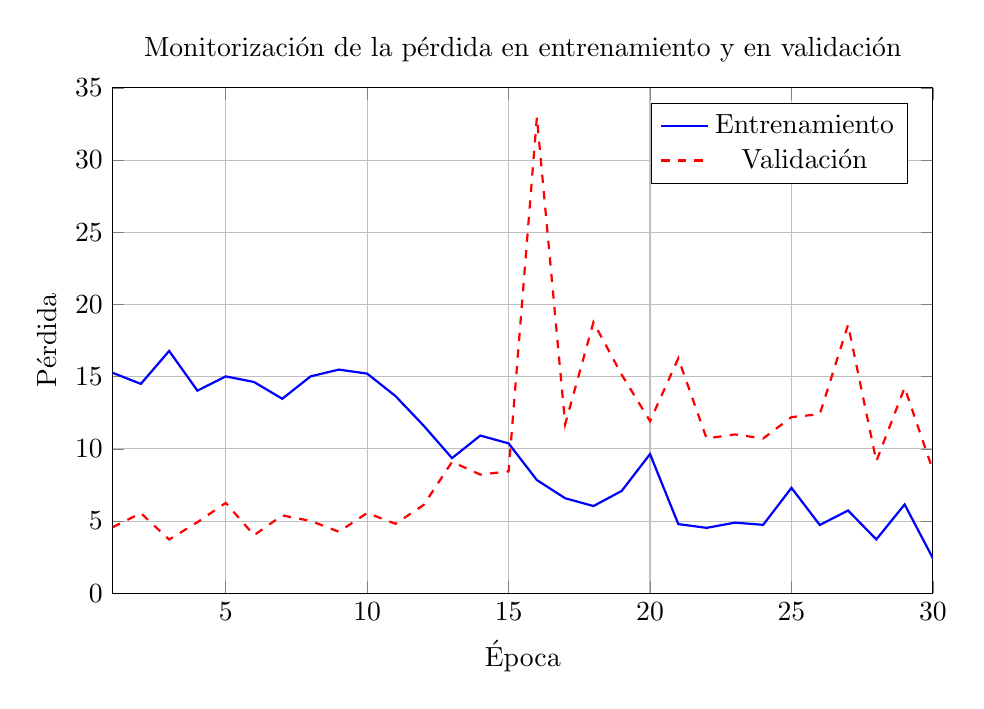
\begin{tikzpicture}
\begin{axis}[
    width=12cm,
    height=8cm,
    xlabel={Época},
    ylabel={Pérdida},
    legend pos=north east,
    grid=both,
    title={Monitorización de la pérdida en entrenamiento y en validación},
    xmin=1, xmax=30,
    ymin=0, ymax=35,
    xtick={0,5,...,30},
    ytick={0,5,...,35}
]

\addplot[
    color=blue,
    thick
] coordinates {
(1,15.27) (2,14.50) (3,16.78) (4,14.03) (5,15.02)
(6,14.63) (7,13.47) (8,15.02) (9,15.49) (10,15.21)
(11,13.66) (12,11.60) (13,9.36) (14,10.92) (15,10.38)
(16,7.84) (17,6.58) (18,6.04) (19,7.09) (20,9.64)
(21,4.79) (22,4.53) (23,4.89) (24,4.74) (25,7.30)
(26,4.73) (27,5.73) (28,3.73) (29,6.15) (30,2.42)
};
\addlegendentry{Entrenamiento}

\addplot[
    color=red,
    dashed,
    thick
] coordinates {
(1,4.57) (2,5.55) (3,3.72) (4,4.92) (5,6.26)
(6,4.02) (7,5.39) (8,5.01) (9,4.26) (10,5.56)
(11,4.81) (12,6.12) (13,9.10) (14,8.22) (15,8.44)
(16,32.97) (17,11.71) (18,18.77) (19,15.13) (20,11.92)
(21,16.27) (22,10.72) (23,11.00) (24,10.72) (25,12.20)
(26,12.40) (27,18.59) (28,9.15) (29,14.24) (30,8.51)
};
\addlegendentry{Validación}

\end{axis}
\end{tikzpicture}
\caption{Evolución de la pérdida por época en el Fold 3 del mejor experimento de deep learning (G-Mean en test 0.691).}
\label{tab:loss-epoca}
\end{figure}


%----------------------------------

\begin{figure}[!htbp]
\centering
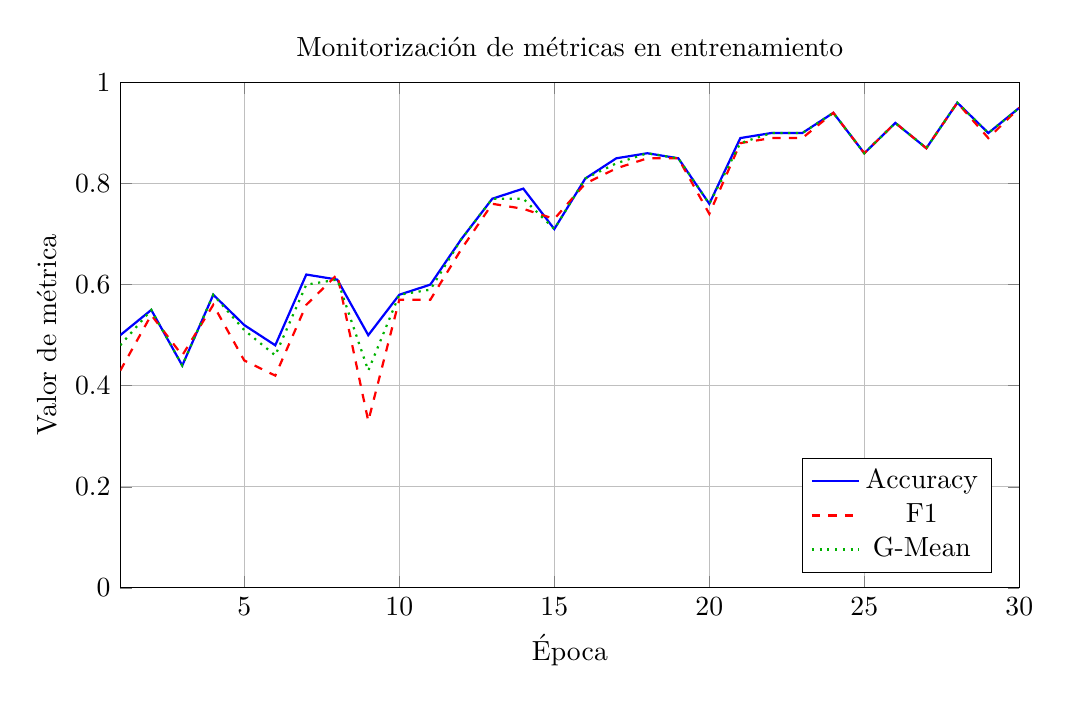
\begin{tikzpicture}
\begin{axis}[
    width=13cm,
    height=8cm,
    xlabel={Época},
    ylabel={Valor de métrica},
    legend pos=south east,
    grid=both,
    title={Monitorización de métricas en entrenamiento},
    xmin=1, xmax=30,
    ymin=0, ymax=1,
    xtick={0,5,...,30},
    ytick={0,0.2,...,1}
]

\addplot[color=blue, thick] coordinates {
(1,0.50) (2,0.55) (3,0.44) (4,0.58) (5,0.52)
(6,0.48) (7,0.62) (8,0.61) (9,0.50) (10,0.58)
(11,0.60) (12,0.69) (13,0.77) (14,0.79) (15,0.71)
(16,0.81) (17,0.85) (18,0.86) (19,0.85) (20,0.76)
(21,0.89) (22,0.90) (23,0.90) (24,0.94) (25,0.86)
(26,0.92) (27,0.87) (28,0.96) (29,0.90) (30,0.95)
};
\addlegendentry{Accuracy}

\addplot[color=red, thick, dashed] coordinates {
(1,0.43) (2,0.54) (3,0.46) (4,0.56) (5,0.45)
(6,0.42) (7,0.56) (8,0.62) (9,0.33) (10,0.57)
(11,0.57) (12,0.67) (13,0.76) (14,0.75) (15,0.73)
(16,0.80) (17,0.83) (18,0.85) (19,0.85) (20,0.74)
(21,0.88) (22,0.89) (23,0.89) (24,0.94) (25,0.86)
(26,0.92) (27,0.87) (28,0.96) (29,0.89) (30,0.95)
};
\addlegendentry{F1}

\addplot[color=green!70!black, thick, dotted] coordinates {
(1,0.48) (2,0.55) (3,0.44) (4,0.58) (5,0.51)
(6,0.46) (7,0.60) (8,0.61) (9,0.43) (10,0.58)
(11,0.59) (12,0.69) (13,0.77) (14,0.77) (15,0.71)
(16,0.81) (17,0.84) (18,0.86) (19,0.85) (20,0.76)
(21,0.88) (22,0.90) (23,0.90) (24,0.94) (25,0.86)
(26,0.92) (27,0.87) (28,0.96) (29,0.90) (30,0.95)
};
\addlegendentry{G-Mean}

\end{axis}
\end{tikzpicture}
\caption{Evolución por época de las métricas en el entrenamiento del Fold 3. Mejor experimento de deep learning (G-Mean en test 0.691).}
\label{tab:train-metricas}
\end{figure}

\begin{figure}[!htbp]
\centering
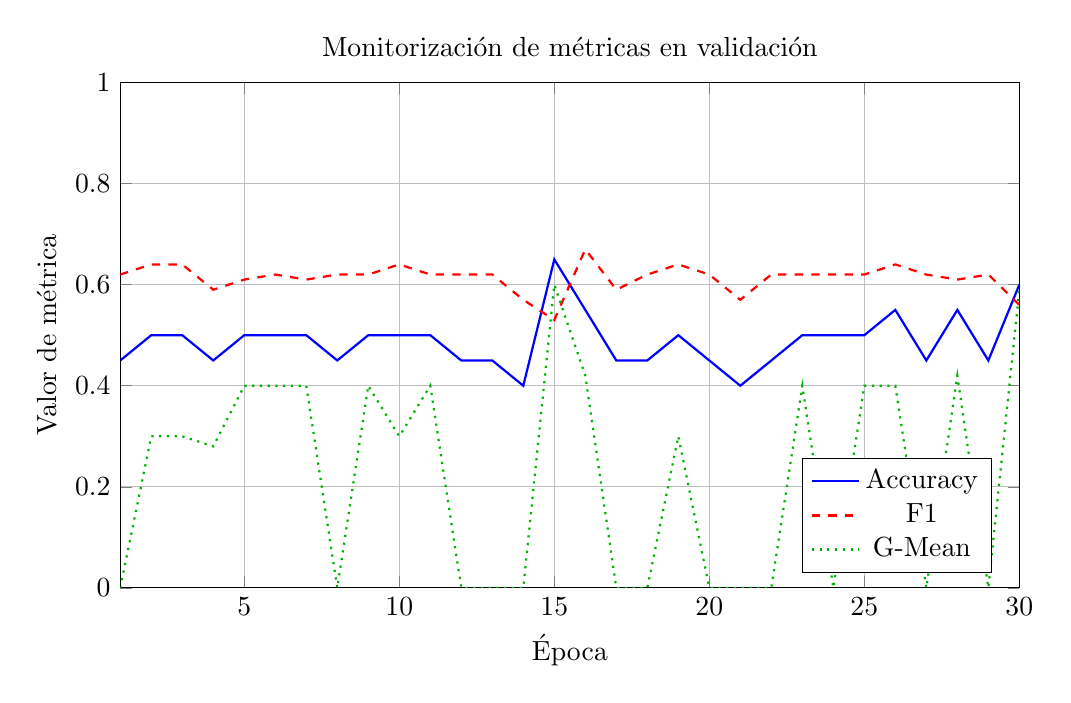
\begin{tikzpicture}
\begin{axis}[
   width=13cm,
    height=8cm,
    xlabel={Época},
    ylabel={Valor de métrica},
    legend pos=south east,
    grid=both,
    title={Monitorización de métricas en validación},
    xmin=1, xmax=30,
    ymin=0, ymax=1,
    xtick={0,5,...,30},
    ytick={0,0.2,...,1}
]

\addplot[color=blue, thick] coordinates {
(1,0.45) (2,0.50) (3,0.50) (4,0.45) (5,0.50)
(6,0.50) (7,0.50) (8,0.45) (9,0.50) (10,0.50)
(11,0.50) (12,0.45) (13,0.45) (14,0.40) (15,0.65)
(16,0.55) (17,0.45) (18,0.45) (19,0.50) (20,0.45)
(21,0.40) (22,0.45) (23,0.50) (24,0.50) (25,0.50)
(26,0.55) (27,0.45) (28,0.55) (29,0.45) (30,0.60)
};
\addlegendentry{Accuracy}

\addplot[color=red, thick, dashed] coordinates {
(1,0.62) (2,0.64) (3,0.64) (4,0.59) (5,0.61)
(6,0.62) (7,0.61) (8,0.62) (9,0.62) (10,0.64)
(11,0.62) (12,0.62) (13,0.62) (14,0.57) (15,0.53)
(16,0.67) (17,0.59) (18,0.62) (19,0.64) (20,0.62)
(21,0.57) (22,0.62) (23,0.62) (24,0.62) (25,0.62)
(26,0.64) (27,0.62) (28,0.61) (29,0.62) (30,0.56)
};
\addlegendentry{F1}

\addplot[color=green!70!black, thick, dotted] coordinates {
(1,0.00) (2,0.30) (3,0.30) (4,0.28) (5,0.40)
(6,0.40) (7,0.40) (8,0.00) (9,0.40) (10,0.30)
(11,0.40) (12,0.00) (13,0.00) (14,0.00) (15,0.60)
(16,0.42) (17,0.00) (18,0.00) (19,0.30) (20,0.00)
(21,0.00) (22,0.00) (23,0.40) (24,0.00) (25,0.40)
(26,0.40) (27,0.00) (28,0.42) (29,0.00) (30,0.59)
};
\addlegendentry{G-Mean}

\end{axis}
\end{tikzpicture}
\caption{Evolución por época de las métricas en el validación del Fold 3. Mejor experimento de deep learning (G-Mean en test 0.691).}
\label{tab:val-metricas}
\end{figure}


\begin{table}[!htbp]
\centering
\caption{Resultados con DenseNet121 medios en test y validación del modelo híbrido (datos y volúmenes) para cada configuración ordenados por G-Mean.}
\label{tab:resultados-hibrido}
\resizebox{\textwidth}{!}{%
\begin{tabular}{lcccccccccccc}
\toprule
\textbf{Set} & \textbf{Batch Size} & \textbf{LR} & \textbf{Weight Decay} & \textbf{Dropout} & \textbf{Preprocesado} & \textbf{Accuracy} & \textbf{F1} & \textbf{TPR} & \textbf{TNR} & \textbf{G-Mean} \\
\midrule
TEST & 4 & 0.001 & 0 & 0.4 & (64,64,64) HU [-1000,400] & 0.512 & 0.459 & 0.456 & 0.559 & 0.469 \\
VALIDATION & 4 & 0.001 & 0 & 0.4 & (64,64,64) HU [-1000,400] & 0.730 & 0.700 & 0.700 & 0.760 & 0.721 \\
\midrule
TEST & 4 & 0.001 & 0 & 0.4 & (64,64,64) HU [-1350,150] & 0.488 & 0.460 & 0.458 & 0.515 & 0.448 \\
VALIDATION & 4 & 0.001 & 0 & 0.4 & (64,64,64) HU [-1350,150] & 0.710 & 0.686 & 0.700 & 0.724 & 0.706 \\
\midrule
TEST & 16 & 0.001 & 0 & 0.4 & (64,64,64) HU [-1000,400] & 0.480 & 0.545 & 0.700 & 0.288 & 0.428 \\
VALIDATION & 16 & 0.001 & 0 & 0.4 & (64,64,64) HU [-1000,400] & 0.660 & 0.679 & 0.784 & 0.556 & 0.618 \\
\midrule
TEST & 16 & 0.001 & 0 & 0.4 & (64,64,64) HU [-1350,150] & 0.496 & 0.552 & 0.662 & 0.344 & 0.413 \\
VALIDATION & 16 & 0.001 & 0 & 0.4 & (64,64,64) HU [-1350,150] & 0.650 & 0.685 & 0.807 & 0.520 & 0.561 \\
\midrule
TEST & 4 & 0.0001 & 0 & 0.4 & (64,64,64) HU [-1350,150] & 0.552 & 0.632 & 0.833 & 0.297 & 0.347 \\
VALIDATION & 4 & 0.0001 & 0 & 0.4 & (64,64,64) HU [-1350,150] & 0.570 & 0.651 & 0.871 & 0.316 & 0.369 \\
\midrule
TEST & 4 & 0.0001 & 0 & 0.4 & (64,64,64) HU [-1000,400] & 0.504 & 0.565 & 0.761 & 0.268 & 0.259 \\
VALIDATION & 4 & 0.0001 & 0 & 0.4 & (64,64,64) HU [-1000,400] & 0.500 & 0.550 & 0.722 & 0.318 & 0.340 \\
\midrule
TEST & 16 & 0.0001 & 0 & 0.4 & (64,64,64) HU [-1350,150] & 0.520 & 0.560 & 0.818 & 0.231 & 0.139 \\
VALIDATION & 16 & 0.0001 & 0 & 0.4 & (64,64,64) HU [-1350,150] & 0.480 & 0.506 & 0.800 & 0.236 & 0.085 \\
\midrule
TEST & 16 & 0.0001 & 0 & 0.4 & (64,64,64) HU [-1000,400] & 0.488 & 0.515 & 0.800 & 0.214 & 0.053 \\
VALIDATION & 16 & 0.0001 & 0 & 0.4 & (64,64,64) HU [-1000,400] & 0.510 & 0.521 & 0.800 & 0.260 & 0.110 \\

\bottomrule
\end{tabular}%
}
\end{table}



\begin{sidewaystable}[!htbp]
\centering
\caption{Resultados en test para configuraciones con fine-tuning, validación cruzada con k=5 y distintas funciones de pérdida ordenados por G-Mean.}
\label{tab:resultados-test-frozen}
\resizebox{\textwidth}{!}{%
\begin{tabular}{lcccccccccccccccccc}
\toprule
\textbf{Set} & \textbf{Dataset} & \textbf{Modelo} & \textbf{Fine Tune} & \textbf{Batch Size} & \textbf{LR} & \textbf{Weight Decay} & \textbf{Dropout} & \textbf{Pretrained Size} & \textbf{Preprocesado} & \textbf{Loss} & \textbf{Stop Criterion} & \textbf{Accuracy} & \textbf{F1} & \textbf{TPR} & \textbf{TNR} & \textbf{G-Mean} \\
\midrule
TEST & nodulemnist3d & ResNet3D & descongelado & 16 & 1e-4 & 1e-5 & 0 & (64,64,64) & (64,64,64) HU[-1000,400] & CrossEntropyLoss+ContrastiveLoss & pérdida & 0.5920 & 0.5995 & 0.6637 & 0.5330 & 0.5792 \\
TEST & nodulemnist3d & DenseNet121 & descongelado & 16 & 1e-4 & 1e-5 & 0 & (64,64,64) & (64,64,64) HU[-1000,400] & CrossEntropyLoss & pérdida & 0.5840 & 0.5810 & 0.6288 & 0.5462 & 0.5792 \\
TEST & nodulemnist3d & ResNet3D & descongelado& 16 & 1e-4 & 1e-5 & 0 & (64,64,64) & (64,64,64) HU[-1000,400] & CrossEntropyLoss+TripletLoss & pérdida & 0.5920 & 0.5956 & 0.6788 & 0.5176 & 0.5695 \\
TEST & organmnist3d & DenseNet121 & congelado & 16 & 1e-4 & 1e-5 & 0.3 & (64,64,64) & (64,64,64) HU[-1000,400] & CrossEntropyLoss+TripletLoss & accuracy & 0.5840 & 0.5990 & 0.6621 & 0.5143 & 0.5660 \\
TEST & nodulemnist3d & DenseNet121 & descongelado & 16 & 1e-4 & 1e-5 & 0 & (64,64,64) & (64,64,64) HU[-1000,400] & CrossEntropyLoss+ContrastiveLoss & pérdida & 0.5760 & 0.5861 & 0.6455 & 0.5176 & 0.5580 \\
TEST & nodulemnist3d & ResNet3D & descongelado & 16 & 1e-4 & 1e-5 & 0 & (64,64,64) & (64,64,64) HU[-1000,400] & CrossEntropyLoss+ContrastiveLoss & pérdida & 0.5840 & 0.5374 & 0.5606 & 0.6077 & 0.5566 \\
TEST & organmnist3d & DenseNet121 & congelado & 16 & 1e-4 & 1e-5 & 0.3 & (64,64,64) & (64,64,64) HU[-1000,400] & CrossEntropyLoss+TripletLoss+ContrastiveLoss & pérdida & 0.5840 & 0.5769 & 0.6409 & 0.5264 & 0.5554 \\
TEST & nodulemnist3d & DenseNet121 & congelado & 16 & 1e-4 & 1e-5 & 0 & (64,64,64) & (64,64,64) HU[-1000,400] & CrossEntropyLoss & pérdida & 0.5600 & 0.5314 & 0.5455 & 0.5769 & 0.5545 \\
TEST & nodulemnist3d & ResNet3D & descongelado & 16 & 1e-4 & 1e-5 & 0 & (64,64,64) & (64,64,64) HU[-1000,400] & CrossEntropyLoss+TripletLoss+ContrastiveLoss & accuracy & 0.5840 & 0.5540 & 0.5955 & 0.5747 & 0.5538 \\
TEST & organmnist3d & DenseNet121 & descongelado & 16 & 1e-4 & 1e-5 & 0.3 & (64,64,64) & (64,64,64) HU[-1000,400] & CrossEntropyLoss+ContrastiveLoss & pérdida & 0.5600 & 0.6089 & 0.7303 & 0.4088 & 0.5428 \\
TEST & organmnist3d & DenseNet121 & descongelado & 16 & 1e-4 & 1e-5 & 0.3 & (64,64,64) & (64,64,64) HU[-1000,400] & CrossEntropyLoss+TripletLoss & pérdida & 0.5440 & 0.5207 & 0.5258 & 0.5615 & 0.5422 \\
TEST & organmnist3d & DenseNet121 & congelado & 16 & 1e-4 & 1e-5 & 0.3 & (64,64,64) & (64,64,64) HU[-1000,400] & ContrastiveLoss & pérdida & 0.5760 & 0.5310 & 0.5621 & 0.5934 & 0.5383 \\
TEST & nodulemnist3d & DenseNet121 & congelado & 16 & 1e-4 & 1e-5 & 0 & (64,64,64) & (64,64,64) HU[-1000,400] & CrossEntropyLoss & pérdida & 0.5520 & 0.4912 & 0.4606 & 0.6374 & 0.5380 \\
TEST & nodulemnist3d & DenseNet121 & congelado & 16 & 1e-4 & 1e-5 & 0.3 & (64,64,64) & (64,64,64) HU[-1000,400] & CrossEntropyLoss+TripletLoss & pérdida & 0.5600 & 0.5389 & 0.5636 & 0.5659 & 0.5377 \\
TEST & nodulemnist3d & DenseNet121 & descongelado & 16 & 1e-4 & 1e-5 & 0 & (64,64,64) & (64,64,64) HU[-1000,400] & CrossEntropyLoss+ContrastiveLoss & pérdida & 0.5680 & 0.5507 & 0.6106 & 0.5330 & 0.5361 \\
TEST & nodulemnist3d & ResNet3D & descongelado & 16 & 1e-4 & 1e-5 & 0 & (64,64,64) & (64,64,64) HU[-1000,400] & CrossEntropyLoss+TripletLoss & pérdida & 0.5600 & 0.5576 & 0.6136 & 0.5198 & 0.5346 \\
TEST & nodulemnist3d & ResNet3D & descongelado & 16 & 1e-4 & 1e-5 & 0 & (64,64,64) & (64,64,64) HU[-1000,400] & CrossEntropyLoss+TripletLoss+ContrastiveLoss & pérdida & 0.5600 & 0.5175 & 0.5106 & 0.6088 & 0.5338 \\
TEST & nodulemnist3d & ResNet3D & congelado & 16 & 1e-4 & 1e-5 & 0 & (64,64,64) & (64,64,64) HU[-1000,400] & CrossEntropyLoss+ContrastiveLoss & pérdida & 0.5600 & 0.5429 & 0.5954 & 0.5341 & 0.5313 \\
TEST & nodulemnist3d & ResNet3D & congelado & 16 & 1e-4 & 1e-5 & 0 & (64,64,64) & (64,64,64) HU[-1000,400] & CrossEntropyLoss+TripletLoss & accuracy & 0.5520 & 0.4961 & 0.4773 & 0.6242 & 0.5313 \\
TEST & organmnist3d & DenseNet121 & descongelado & 16 & 1e-4 & 1e-5 & 0.3 & (64,64,64) & (64,64,64) HU[-1000,400] & ContrastiveLoss & pérdida & 0.5520 & 0.5240 & 0.5545 & 0.5462 & 0.5272 \\
TEST & nodulemnist3d & DenseNet121 & congelado & 16 & 1e-4 & 1e-5 & 0.3 & (64,64,64) & (64,64,64) HU[-1000,400] & CrossEntropyLoss+TripletLoss & pérdida & 0.5520 & 0.5856 & 0.6803 & 0.4418 & 0.5256 \\
TEST & organmnist3d & DenseNet121 & congelado & 16 & 1e-4 & 1e-5 & 0.3 & (64,64,64) & (64,64,64) HU[-1000,400] & CrossEntropyLoss+TripletLoss & pérdida & 0.5840 & 0.4775 & 0.4394 & 0.7121 & 0.5255 \\
TEST & organmnist3d & DenseNet121 & congelado & 16 & 1e-4 & 1e-5 & 0.3 & (64,64,64) & (64,64,64) HU[-1000,400] & ContrastiveLoss & accuracy & 0.5360 & 0.5292 & 0.5818 & 0.4978 & 0.5236 \\
TEST & organmnist3d & DenseNet121 & congelado & 16 & 1e-4 & 1e-5 & 0.3 & (64,64,64) & (64,64,64) HU[-1000,400] & CrossEntropyLoss+ContrastiveLoss & pérdida & 0.5600 & 0.6068 & 0.7303 & 0.4077 & 0.5233 \\
TEST & organmnist3d & DenseNet121 & descongelado & 16 & 1e-4 & 1e-5 & 0.3 & (64,64,64) & (64,64,64) HU[-1000,400] & CrossEntropyLoss+TripletLoss+ContrastiveLoss & pérdida & 0.5520 & 0.5386 & 0.5742 & 0.5275 & 0.5219 \\
TEST & nodulemnist3d & DenseNet121 & congelado & 16 & 1e-4 & 1e-5 & 0 & (64,64,64) & (64,64,64) HU[-1000,400] & CrossEntropyLoss+ContrastiveLoss & pérdida & 0.5360 & 0.5530 & 0.6106 & 0.4714 & 0.5191 \\
TEST & nodulemnist3d & DenseNet121 & congelado & 16 & 1e-4 & 1e-5 & 0.3 & (64,64,64) & (64,64,64) HU[-1000,400] & CrossEntropyLoss+ContrastiveLoss & pérdida & 0.5440 & 0.4702 & 0.4424 & 0.6352 & 0.5165 \\
TEST & nodulemnist3d & ResNet3D & descongelado & 16 & 1e-4 & 1e-5 & 0 & (64,64,64) & (64,64,64) HU[-1000,400] & CrossEntropyLoss & pérdida & 0.5280 & 0.5494 & 0.6227 & 0.4396 & 0.5161 \\
TEST & nodulemnist3d & DenseNet121 & congelado & 16 & 1e-4 & 1e-5 & 0 & (64,64,64) & (64,64,64) HU[-1000,400] & CrossEntropyLoss+TripletLoss & pérdida & 0.5280 & 0.4889 & 0.4924 & 0.5626 & 0.5152 \\
TEST & organmnist3d & DenseNet121 & descongelado & 16 & 1e-4 & 1e-5 & 0.3 & (64,64,64) & (64,64,64) HU[-1000,400] & CrossEntropyLoss+ContrastiveLoss & pérdida & 0.5520 & 0.5743 & 0.6667 & 0.4593 & 0.5146 \\
TEST & organmnist3d & DenseNet121 & congelado & 16 & 1e-4 & 1e-5 & 0.3 & (64,64,64) & (64,64,64) HU[-1000,400] & CrossEntropyLoss+TripletLoss & accuracy & 0.5520 & 0.5842 & 0.7167 & 0.4110 & 0.5135 \\
TEST & nodulemnist3d & ResNet3D & descongelado & 16 & 1e-4 & 1e-5 & 0 & (64,64,64) & (64,64,64) HU[-1000,400] & CrossEntropyLoss+TripletLoss+ContrastiveLoss & accuracy & 0.5440 & 0.5598 & 0.6258 & 0.4714 & 0.5135 \\
TEST & organmnist3d & DenseNet121 & descongelado & 16 & 1e-4 & 1e-5 & 0.3 & (64,64,64) & (64,64,64) HU[-1000,400] & CrossEntropyLoss+TripletLoss+ContrastiveLoss & accuracy & 0.5440 & 0.4824 & 0.4742 & 0.6044 & 0.5093 \\
TEST & nodulemnist3d & DenseNet121 & descongelado & 16 & 1e-4 & 1e-5 & 0 & (64,64,64) & (64,64,64) HU[-1000,400] & TripletLoss & pérdida & 0.5200 & 0.5316 & 0.5939 & 0.4560 & 0.5081 \\
TEST & organmnist3d & DenseNet121 & descongelado & 16 & 1e-4 & 1e-5 & 0.3 & (64,64,64) & (64,64,64) HU[-1000,400] & ContrastiveLoss & pérdida & 0.5920 & 0.4326 & 0.3712 & 0.7868 & 0.5074 \\
TEST & organmnist3d & DenseNet121 & congelado & 16 & 1e-4 & 1e-5 & 0.3 & (64,64,64) & (64,64,64) HU[-1000,400] & ContrastiveLoss & pérdida & 0.5600 & 0.5115 & 0.5743 & 0.5473 & 0.5055 \\
TEST & nodulemnist3d & DenseNet121 & descongelado & 16 & 1e-4 & 1e-5 & 0 & (64,64,64) & (64,64,64) HU[-1000,400] & CrossEntropyLoss+TripletLoss & pérdida & 0.5440 & 0.4921 & 0.4894 & 0.5901 & 0.5046 \\
TEST & organmnist3d & DenseNet121 & descongelado & 16 & 1e-4 & 1e-5 & 0.3 & (64,64,64) & (64,64,64) HU[-1000,400] & CrossEntropyLoss & accuracy & 0.5520 & 0.4398 & 0.4242 & 0.6671 & 0.5014 \\
TEST & organmnist3d & DenseNet121 & descongelado & 16 & 1e-4 & 1e-5 & 0.3 & (64,64,64) & (64,64,64) HU[-1000,400] & CrossEntropyLoss+TripletLoss+ContrastiveLoss & pérdida & 0.5040 & 0.4959 & 0.5258 & 0.4835 & 0.5003 \\
TEST & organmnist3d & DenseNet121 & congelado & 16 & 1e-4 & 1e-5 & 0.3 & (64,64,64) & (64,64,64) HU[-1000,400] & CrossEntropyLoss+ContrastiveLoss & accuracy & 0.5520 & 0.4641 & 0.4757 & 0.6253 & 0.5002 \\
\bottomrule
\end{tabular}%
}
\end{sidewaystable}



\begin{table}[!htbp]
\centering
\caption{Resultados medios solo con los datos clínicos en test para KNN (5-fold Cross-Validation) ordenados por G-Mean.}
\label{tab:resultados-knn}
\resizebox{\textwidth}{!}{%
\begin{tabular}{ccccccccc}
\toprule
\textbf{n\_neighbors} & \textbf{weights} & \textbf{metric} & \textbf{Accuracy} & \textbf{F1} & \textbf{TPR} & \textbf{TNR} & \textbf{G-Mean} \\
\midrule
5 & uniform & euclidean & 0.520 & 0.497 & 0.509 & 0.533 & 0.509 \\
3 & uniform & euclidean & 0.512 & 0.476 & 0.474 & 0.547 & 0.503 \\
7 & uniform & manhattan & 0.512 & 0.468 & 0.458 & 0.563 & 0.503 \\
5 & distance & euclidean & 0.480 & 0.466 & 0.476 & 0.487 & 0.478 \\
9 & distance & manhattan & 0.480 & 0.404 & 0.374 & 0.577 & 0.452 \\
\bottomrule
\end{tabular}%
}
\end{table}

\begin{table}[!htbp]
\centering
\caption{Resultados medios solo con los datos clínicos en test para Random Forest (5-fold Cross-Validation) ordenados por G-Mean.}
\label{tab:resultados-rf}
\resizebox{\textwidth}{!}{%
\begin{tabular}{ccccccccc}
\toprule
\textbf{n\_estimators} & \textbf{max\_depth} & \textbf{min\_samples\_split} & \textbf{Accuracy} & \textbf{F1} & \textbf{TPR} & \textbf{TNR} & \textbf{G-Mean} \\
\midrule
100 & 5 & 2 & 0.552 & 0.443 & 0.373 & 0.712 & 0.515 \\
200 & 10 & 4 & 0.536 & 0.442 & 0.392 & 0.665 & 0.508 \\
300 & None & 2 & 0.504 & 0.443 & 0.424 & 0.576 & 0.485 \\
\bottomrule
\end{tabular}%
}
\end{table}


\begin{table}[!htbp]
\centering
\caption{Resultados medios solo con los datos clínicos en test para LightGBM (5-fold Cross-Validation) ordenados por G-Mean.}
\label{tab:resultados-lightgbm}
\resizebox{\textwidth}{!}{%
\begin{tabular}{ccccccccc}
\toprule
\textbf{n\_estimators} & \textbf{max\_depth} & \textbf{learning\_rate} & \textbf{Accuracy} & \textbf{F1} & \textbf{TPR} & \textbf{TNR} & \textbf{G-Mean} \\
\midrule
200 & 6 & 0.05 & 0.552 & 0.473 & 0.426 & 0.667 & 0.531 \\
100 & 4 & 0.1 & 0.544 & 0.477 & 0.442 & 0.637 & 0.528 \\
300 & 8 & 0.03 & 0.544 & 0.468 & 0.426 & 0.653 & 0.524 \\
\bottomrule
\end{tabular}%
}
\end{table}

\begin{table}[!htbp]
\centering
\caption{Resultados medios solo con los datos clínicos en test para XGBoost (5-fold Cross-Validation) ordenados por G-Mean.}
\label{tab:resultados-xgboost}
\begin{tabular}{cccccccc}
\toprule
\textbf{n\_estimators} & \textbf{max\_depth} & \textbf{learning\_rate} & \textbf{Accuracy} & \textbf{F1} & \textbf{TPR} & \textbf{TNR} & \textbf{G-Mean} \\
\midrule
400 & 6  & 0.01 & 0.576 & 0.498 & 0.444 & 0.695 & 0.553 \\
200 & 5  & 0.05 & 0.568 & 0.503 & 0.461 & 0.664 & 0.552 \\
350 & 12 & 0.02 & 0.568 & 0.494 & 0.444 & 0.679 & 0.548 \\
300 & 8  & 0.02 & 0.568 & 0.494 & 0.444 & 0.679 & 0.548 \\
300 & 8  & 0.03 & 0.560 & 0.489 & 0.444 & 0.679 & 0.547 \\
150 & 8  & 0.07 & 0.560 & 0.489 & 0.442 & 0.664 & 0.540 \\
250 & 10 & 0.05 & 0.560 & 0.479 & 0.426 & 0.679 & 0.534 \\
100 & 4  & 0.1  & 0.552 & 0.480 & 0.444 & 0.651 & 0.534 \\
100 & 3  & 0.2  & 0.536 & 0.455 & 0.408 & 0.649 & 0.512 \\
\bottomrule
\end{tabular}
\end{table}


\begin{sidewaystable}[!htbp]
\centering
\caption{Resultados medios en test de radiómica sin datos clínicos y sin DML para distintos modelos con 5-fold Cross-Validation ordenados por G-Mean. Todas las características son extendidas.}
\label{tab:resultados-clasificadores}
\resizebox{\textwidth}{!}{%
\begin{tabular}{ccccccccccc}
\toprule
\textbf{Modelo} & \textbf{Parámetros} & \textbf{Scaler} & \textbf{Preprocesado} & \textbf{Reducción de dimensionalidad} & \textbf{Accuracy} & \textbf{F1} & \textbf{TPR} & \textbf{TNR} & \textbf{G-Mean} \\
\midrule
KNN & n\_neighbors=5, weights=distance & StandardScaler & (128,128,128), HU [-1350,150] & - & 0.744 & 0.713 & 0.724 & 0.765 & 0.739 \\
LightGBM & n\_estimators=200, learning\_rate=0.1, num\_leaves=31 & - & (28,28,28), HU [-1350,150] & Variance Threshold (0.01) & 0.744 & 0.703 & 0.680 & 0.791 & 0.728 \\
KNN & n\_neighbors=5, weights=distance & - & (128,128,128), HU [-1350,150] & PCA (99\%) & 0.736 & 0.692 & 0.688 & 0.779 & 0.724 \\
KNN & n\_neighbors=7, weights=distance & MinMaxScaler & (128,256,256), HU [-1350,150] & - & 0.728 & 0.711 & 0.688 & 0.766 & 0.719 \\
KNN & n\_neighbors=5, weights=uniform & StandardScaler & (128,128,128), HU [-1350,150] & - & 0.720 & 0.679 & 0.724 & 0.721 & 0.716 \\
KNN & n\_neighbors=7, weights=distance & - & (128,128,128), HU [-1350,150] & Variance Threshold (0.01) & 0.712 & 0.702 & 0.741 & 0.692 & 0.711 \\
KNN & n\_neighbors=7, weights=distance & - & (128,128,128), HU [-1350,150] & - & 0.712 & 0.702 & 0.741 & 0.692 & 0.711 \\
KNN & n\_neighbors=7, weights=distance & MinMaxScaler & (128,128,128), HU [-1000,400] & PCA (90\%) & 0.712 & 0.706 & 0.756 & 0.674 & 0.709 \\
LightGBM & n\_estimators=100, learning\_rate=0.1, num\_leaves=50 & StandardScaler & (28,28,28), HU [-1350,150] & Variance Threshold (0.01) & 0.728 & 0.679 & 0.645 & 0.791 & 0.708 \\
LightGBM & n\_estimators=50, learning\_rate=0.1, num\_leaves=50 & StandardScaler & (28,28,28), HU [-1350,150] & Variance Threshold (0.01) & 0.720 & 0.676 & 0.647 & 0.777 & 0.705 \\
SVM & C=10.0, kernel=rbf, gamma=scale & - & (128,256,256), HU [-1000,400] & PCA (99\%) & 0.712 & 0.683 & 0.688 & 0.735 & 0.704 \\
LightGBM & n\_estimators=100, learning\_rate=0.1, num\_leaves=50 & - & (28,28,28), HU [-1350,150] & Variance Threshold (0.01) & 0.712 & 0.681 & 0.682 & 0.733 & 0.703 \\
SVM & C=10.0, kernel=rbf, gamma=scale & - & (128,256,256), HU [-1000,400] & PCA (95\%) & 0.712 & 0.683 & 0.688 & 0.734 & 0.702 \\
KNN & n\_neighbors=5, weights=uniform & - & (128,128,128), HU [-1350,150] & PCA (99\%) & 0.712 & 0.673 & 0.688 & 0.735 & 0.702 \\
KNN & n\_neighbors=3, weights=distance & StandardScaler & (128,128,128), HU [-1000,400] & Variance Threshold (0.01) & 0.712 & 0.679 & 0.683 & 0.736 & 0.702 \\
KNN & n\_neighbors=7, weights=distance & - & (128,256,256), HU [-1350,150] & PCA (99\%) & 0.704 & 0.678 & 0.706 & 0.707 & 0.701 \\
KNN & n\_neighbors=7, weights=distance & StandardScaler & (128,128,128), HU [-1000,400] & PCA (95\%) & 0.704 & 0.696 & 0.753 & 0.662 & 0.701 \\
DecisionTree & max\_depth=5, min\_samples\_split=2 & StandardScaler & (128,128,128), HU [-1350,150] & PCA (95\%) & 0.704 & 0.677 & 0.686 & 0.720 & 0.700 \\
KNN & n\_neighbors=7, weights=distance & MinMaxScaler & (128,128,128), HU [-1350,150] & - & 0.712 & 0.664 & 0.653 & 0.765 & 0.700 \\
KNN & n\_neighbors=5, weights=distance & StandardScaler & (128,256,256), HU [-1000,400] & Variance Threshold (0.01) & 0.712 & 0.674 & 0.668 & 0.748 & 0.700 \\
KNN & n\_neighbors=5, weights=distance & MinMaxScaler & (128,128,128), HU [-1350,150] & - & 0.712 & 0.672 & 0.689 & 0.737 & 0.699 \\
KNN & n\_neighbors=7, weights=distance & StandardScaler & (128,128,128), HU [-1000,400] & PCA (90\%) & 0.704 & 0.703 & 0.774 & 0.645 & 0.699 \\
KNN & n\_neighbors=5, weights=distance & - & (128,128,128), HU [-1350,150] & PCA (95\%) & 0.704 & 0.669 & 0.670 & 0.735 & 0.698 \\
LightGBM & n\_estimators=50, learning\_rate=0.1, num\_leaves=31 & - & (28,28,28), HU [-1350,150] & Variance Threshold (0.01) & 0.704 & 0.682 & 0.698 & 0.704 & 0.698 \\
LightGBM & n\_estimators=200, learning\_rate=0.1, num\_leaves=31 & MinMaxScaler & (28,28,28), HU [-1350,150] & Variance Threshold (0.01) & 0.712 & 0.675 & 0.679 & 0.733 & 0.698 \\
KNN & n\_neighbors=5, weights=distance & StandardScaler & (128,128,128), HU [-1350,150] & Variance Threshold (0.01) & 0.712 & 0.670 & 0.667 & 0.752 & 0.698 \\
KNN & n\_neighbors=5, weights=distance & MinMaxScaler & (128,128,128), HU [-1000,400] & PCA (90\%) & 0.704 & 0.675 & 0.667 & 0.733 & 0.698 \\
KNN & n\_neighbors=7, weights=distance & StandardScaler & (128,256,256), HU [-1350,150] & Variance Threshold (0.01) & 0.704 & 0.665 & 0.671 & 0.734 & 0.696 \\
SVM & C=10.0, kernel=rbf, gamma=scale & - & (128,256,256), HU [-1000,400] & PCA (90\%) & 0.696 & 0.687 & 0.738 & 0.662 & 0.695 \\
KNN & n\_neighbors=7, weights=distance & - & (128,128,128), HU [-1000,400] & - & 0.696 & 0.686 & 0.723 & 0.678 & 0.695 \\
KNN & n\_neighbors=5, weights=distance & - & (128,128,128), HU [-1350,150] & PCA (90\%) & 0.704 & 0.664 & 0.670 & 0.735 & 0.694 \\
KNN & n\_neighbors=5, weights=distance & MinMaxScaler & (128,256,256), HU [-1000,400] & PCA (90\%) & 0.696 & 0.673 & 0.683 & 0.705 & 0.693 \\
KNN & n\_neighbors=5, weights=distance & StandardScaler & (128,128,128), HU [-1000,400] & - & 0.696 & 0.670 & 0.686 & 0.704 & 0.693 \\
RandomForest & n\_estimators=50, max\_depth=5, min\_samples\_split=5 & MinMaxScaler & (128,128,128), HU [-1000,400] & PCA (90\%) & 0.704 & 0.668 & 0.633 & 0.763 & 0.692 \\
KNN & n\_neighbors=5, weights=uniform & StandardScaler & (128,128,128), HU [-1350,150] & Variance Threshold (0.01) & 0.704 & 0.663 & 0.667 & 0.737 & 0.692 \\
XGBoost & n\_estimators=100, learning\_rate=0.1, max\_depth=5 & MinMaxScaler & (128,128,128), HU [-1000,400] & PCA (90\%) & 0.704 & 0.667 & 0.667 & 0.736 & 0.692 \\
XGBoost & n\_estimators=100, learning\_rate=0.1, max\_depth=5 & - & (28,28,28), HU [-1350,150] & - & 0.704 & 0.655 & 0.614 & 0.778 & 0.691 \\
KNN & n\_neighbors=7, weights=distance & - & (128,128,128), HU [-1350,150] & PCA (99\%) & 0.712 & 0.648 & 0.618 & 0.793 & 0.690 \\
LightGBM & n\_estimators=100, learning\_rate=0.01, num\_leaves=50 & MinMaxScaler & (128,128,128), HU [-1350,150] & PCA (95\%) & 0.712 & 0.657 & 0.611 & 0.791 & 0.690 \\

\bottomrule
\end{tabular}%
}
\end{sidewaystable}


\begin{sidewaystable}[!htbp]
\centering
\caption{Resultados medios en test de radiómica con datos clínicos y sin DML para distintos modelos con 5-fold Cross-Validation ordenados por G-Mean.}
\label{tab:resultados-clinicos}
\resizebox{\textwidth}{!}{%
\begin{tabular}{ccccccccccc}
\toprule
\textbf{Características} & \textbf{Modelo} & \textbf{Parámetros} & \textbf{Scaler} & \textbf{Preprocesado} & \textbf{Reducción de dimensionalidad} & \textbf{Accuracy} & \textbf{F1} & \textbf{TPR} & \textbf{TNR} & \textbf{G-Mean} \\
\midrule
Extendidas & LightGBM & n\_estimators=100, learning\_rate=0.1, num\_leaves=31 & StandardScaler & (28,28,28), HU [-1350,150] & Variance Threshold (0.01) & 0.760 & 0.725 & 0.700 & 0.805 & 0.746 \\
Originales & GradientBoosting & n\_estimators=200, learning\_rate=0.01, max\_depth=5 & StandardScaler & (256,512,512), HU [-1000,400] & PCA (90\%) & 0.752 & 0.709 & 0.665 & 0.821 & 0.736 \\
Extendidas & KNN & n\_neighbors=5, weights=distance & MinMaxScaler & (128,128,128), HU [-1350,150] & - & 0.728 & 0.684 & 0.689 & 0.766 & 0.712 \\
Extendidas & KNN & n\_neighbors=7, weights=distance & - & (128,128,128), HU [-1350,150] & - & 0.712 & 0.702 & 0.741 & 0.692 & 0.711 \\
Originales & GradientBoosting & n\_estimators=100, learning\_rate=0.01, max\_depth=5 & - & (256,512,512), HU [-1000,400] & PCA (90\%) & 0.728 & 0.673 & 0.614 & 0.822 & 0.709 \\
Originales & XGBoost & n\_estimators=200, learning\_rate=0.1, max\_depth=null & MinMaxScaler & (256,512,512), HU [-1350,150] & - & 0.728 & 0.674 & 0.632 & 0.808 & 0.707 \\
Extendidas & LightGBM & n\_estimators=200, learning\_rate=0.1, num\_leaves=50 & StandardScaler & (28,28,28), HU [-1350,150] & Variance Threshold (0.01) & 0.736 & 0.678 & 0.644 & 0.805 & 0.707 \\
Extendidas & LightGBM & n\_estimators=50, learning\_rate=0.1, num\_leaves=31 & StandardScaler & (28,28,28), HU [-1350,150] & Variance Threshold (0.01) & 0.720 & 0.676 & 0.647 & 0.777 & 0.705 \\
Extendidas & KNN & n\_neighbors=5, weights=uniform & MinMaxScaler & (128,128,128), HU [-1350,150] & - & 0.720 & 0.678 & 0.689 & 0.752 & 0.705 \\
Originales & XGBoost & n\_estimators=100, learning\_rate=0.1, max\_depth=null & - & (256,512,512), HU [-1350,150] & - & 0.720 & 0.666 & 0.632 & 0.793 & 0.701 \\
Extendidas & RandomForest & n\_estimators=200, max\_depth=10, min\_samples\_split=2 & - & (128,128,128), HU [-1000,400] & PCA (90\%) & 0.720 & 0.667 & 0.612 & 0.808 & 0.700 \\
Originales & XGBoost & n\_estimators=200, learning\_rate=0.1, max\_depth=5 & - & (256,512,512), HU [-1350,150] & - & 0.712 & 0.667 & 0.650 & 0.764 & 0.699 \\
Originales & GradientBoosting & n\_estimators=100, learning\_rate=0.01, max\_depth=5 & - & (256,512,512), HU [-1350,150] & - & 0.720 & 0.666 & 0.598 & 0.820 & 0.699 \\
Extendidas & LightGBM & n\_estimators=200, learning\_rate=0.1, num\_leaves=50 & - & (28,28,28), HU [-1350,150] & Variance Threshold (0.01) & 0.720 & 0.671 & 0.661 & 0.762 & 0.697 \\
Originales & SVM & C=1.0, kernel=rbf, gamma=scale & StandardScaler & (128,128,128), HU [-1350,150] & Variance Threshold (0.01) & 0.720 & 0.663 & 0.615 & 0.808 & 0.697 \\
Originales & GradientBoosting & n\_estimators=200, learning\_rate=0.01, max\_depth=5 & - & (256,512,512), HU [-1350,150] & - & 0.712 & 0.661 & 0.615 & 0.791 & 0.696 \\
Extendidas & RandomForest & n\_estimators=100, max\_depth=10, min\_samples\_split=5 & - & (128,128,128), HU [-1000,400] & PCA (90\%) & 0.720 & 0.659 & 0.595 & 0.822 & 0.695 \\
Originales & GradientBoosting & n\_estimators=50, learning\_rate=0.01, max\_depth=null & StandardScaler & (256,512,512), HU [-1000,400] & PCA (90\%) & 0.712 & 0.662 & 0.614 & 0.793 & 0.695 \\
Extendidas & LightGBM & n\_estimators=50, learning\_rate=0.1, num\_leaves=50 & - & (28,28,28), HU [-1350,150] & Variance Threshold (0.01) & 0.704 & 0.673 & 0.680 & 0.719 & 0.695 \\
Extendidas & KNN & n\_neighbors=7, weights=distance & - & (128,128,128), HU [-1000,400] & - & 0.696 & 0.686 & 0.723 & 0.678 & 0.695 \\
Originales & XGBoost & n\_estimators=50, learning\_rate=0.1, max\_depth=10 & - & (256,512,512), HU [-1000,400] & PCA (95\%) & 0.712 & 0.667 & 0.645 & 0.762 & 0.694 \\
Originales & XGBoost & n\_estimators=50, learning\_rate=0.1, max\_depth=5 & - & (256,512,512), HU [-1350,150] & - & 0.712 & 0.658 & 0.614 & 0.793 & 0.694 \\
Originales & GradientBoosting & n\_estimators=200, learning\_rate=0.1, max\_depth=10 & - & (256,512,512), HU [-1000,400] & PCA (90\%) & 0.704 & 0.665 & 0.648 & 0.748 & 0.692 \\
Originales & XGBoost & n\_estimators=100, learning\_rate=0.1, max\_depth=5 & StandardScaler & (256,512,512), HU [-1350,150] & - & 0.712 & 0.656 & 0.614 & 0.792 & 0.691 \\
Originales & GradientBoosting & n\_estimators=50, learning\_rate=0.01, max\_depth=5 & StandardScaler & (256,512,512), HU [-1000,400] & PCA (90\%) & 0.712 & 0.654 & 0.595 & 0.807 & 0.691 \\
Extendidas & XGBoost & n\_estimators=100, learning\_rate=0.1, max\_depth=10 & StandardScaler & (28,28,28), HU [-1350,150] & Variance Threshold (0.01) & 0.704 & 0.662 & 0.630 & 0.765 & 0.691 \\
Originales & XGBoost & n\_estimators=50, learning\_rate=0.1, max\_depth=10 & StandardScaler & (256,512,512), HU [-1350,150] & - & 0.712 & 0.652 & 0.614 & 0.793 & 0.690 \\
Extendidas & LightGBM & n\_estimators=100, learning\_rate=0.1, num\_leaves=31 & - & (28,28,28), HU [-1350,150] & Variance Threshold (0.01) & 0.704 & 0.665 & 0.662 & 0.733 & 0.690 \\
Originales & XGBoost & n\_estimators=200, learning\_rate=0.1, max\_depth=5 & StandardScaler & (256,512,512), HU [-1000,400] & PCA (95\%) & 0.712 & 0.655 & 0.611 & 0.791 & 0.689 \\
Originales & GradientBoosting & n\_estimators=50, learning\_rate=0.01, max\_depth=5 & - & (256,512,512), HU [-1350,150] & - & 0.704 & 0.659 & 0.630 & 0.763 & 0.689 \\
Extendidas & XGBoost & n\_estimators=200, learning\_rate=0.1, max\_depth=10 & StandardScaler & (28,28,28), HU [-1350,150] & Variance Threshold (0.01) & 0.704 & 0.658 & 0.629 & 0.764 & 0.689 \\
Extendidas & XGBoost & n\_estimators=50, learning\_rate=0.01, max\_depth=10 & MinMaxScaler & (128,128,128), HU [-1350,150] & PCA (95\%) & 0.704 & 0.658 & 0.629 & 0.764 & 0.689 \\
\bottomrule
\end{tabular}%
}
\end{sidewaystable}


\begin{sidewaystable}[!htbp]
\centering
\caption{Resultados medios en test de radiómica sin datos clínicos y con DML para KNN con 5-fold Cross-Validation ordenados por G-Mean. Todas las características son extendidas.}
\label{tab:resultados-sindatos-dml}
\resizebox{\textwidth}{!}{%
\begin{tabular}{ccccccccccc}
\toprule
\textbf{Número de vecinos} & \textbf{Weights} & \textbf{Scaler} & \textbf{Preprocesado} & \textbf{Algoritmo DML} & \textbf{Dimensión DML} & \textbf{Accuracy} & \textbf{F1} & \textbf{TPR} & \textbf{TNR} & \textbf{G-Mean} \\
\midrule
5 & distance & StandardScaler & (128,128,128), HU [-1350,150] & nca & all & 0.744 & 0.713 & 0.724 & 0.765 & 0.739 \\
5 & distance & - & (128,128,128), HU [-1350,150] & nca & 20 & 0.736 & 0.707 & 0.723 & 0.749 & 0.732 \\
5 & distance & - & (128,128,128), multiwindowing & lmnn & all & 0.733 & 0.704 & 0.727 & 0.738 & 0.731 \\
7 & distance & StandardScaler & (64,64,64), no HU & lmnn & all & 0.747 & 0.696 & 0.667 & 0.810 & 0.725 \\
5 & uniform & MinMaxScaler & (64,64,64), no HU & lmnn & 10 & 0.728 & 0.697 & 0.688 & 0.766 & 0.721 \\
5 & distance & - & (64,64,64), no HU & lmnn & 20 & 0.752 & 0.686 & 0.598 & 0.880 & 0.721 \\
5 & distance & MinMaxScaler & (64,64,64), no HU & lmnn & 10 & 0.728 & 0.691 & 0.670 & 0.780 & 0.720 \\
3 & distance & - & (128,128,128), HU [-1350,150] & lmnn & all & 0.720 & 0.705 & 0.758 & 0.690 & 0.720 \\
7 & distance & MinMaxScaler & (128,256,256), HU [-1350,150] & nca & all & 0.728 & 0.691 & 0.688 & 0.766 & 0.719 \\
3 & uniform & StandardScaler & (64,64,64), no HU & lmnn & all & 0.733 & 0.676 & 0.636 & 0.810 & 0.717 \\
3 & distance & MinMaxScaler & (64,64,64), no HU & lmnn & 20 & 0.720 & 0.692 & 0.691 & 0.746 & 0.717 \\
3 & uniform & MinMaxScaler & (64,64,64), no HU & lmnn & 20 & 0.720 & 0.692 & 0.691 & 0.746 & 0.717 \\
7 & distance & StandardScaler & (64,64,64), no HU & lmnn & all & 0.720 & 0.692 & 0.689 & 0.747 & 0.716 \\
5 & uniform & StandardScaler & (128,128,128), HU [-1350,150] & nca & all & 0.720 & 0.694 & 0.724 & 0.721 & 0.716 \\
7 & distance & - & (128,128,128), HU [-1350,150] & nca & 30 & 0.712 & 0.702 & 0.741 & 0.692 & 0.711 \\
5 & distance & - & (128,256,256), HU [-1350,150] & nca & 10 & 0.712 & 0.691 & 0.702 & 0.723 & 0.710 \\
7 & uniform & StandardScaler & (64,64,64), no HU & lmnn & all & 0.712 & 0.685 & 0.689 & 0.733 & 0.710 \\
3 & distance & MinMaxScaler & (128,128,128), HU [-1350,150] & lmnn & 30 & 0.710 & 0.686 & 0.710 & 0.710 & 0.709 \\
5 & uniform & - & (128,128,128), HU [-1350,150] & nca & 20 & 0.712 & 0.688 & 0.723 & 0.705 & 0.709 \\
5 & uniform & StandardScaler & (64,64,64), no HU & lmnn & 30 & 0.712 & 0.688 & 0.689 & 0.732 & 0.708 \\
5 & distance & MinMaxScaler & (64,64,64), multiwindowing & lmnn & 20 & 0.720 & 0.678 & 0.646 & 0.779 & 0.708 \\
3 & uniform & - & (64,64,64), no HU & lmnn & 30 & 0.712 & 0.683 & 0.691 & 0.733 & 0.708 \\
3 & uniform & MinMaxScaler & (64,64,64), no HU & lmnn & 30 & 0.712 & 0.688 & 0.689 & 0.732 & 0.707 \\
5 & distance & - & (128,128,128), HU [-1350,150] & nca & 20 & 0.720 & 0.676 & 0.689 & 0.749 & 0.707 \\
7 & distance & MinMaxScaler & (64,64,64), no HU & lmnn & all & 0.733 & 0.673 & 0.636 & 0.810 & 0.707 \\
7 & distance & StandardScaler & (128,256,256), HU [-1000,400] & nca & all & 0.704 & 0.694 & 0.738 & 0.678 & 0.705 \\
7 & uniform & MinMaxScaler & (64,64,64), no HU & lmnn & 30 & 0.712 & 0.681 & 0.671 & 0.747 & 0.705 \\
5 & distance & MinMaxScaler & (128,128,128), no HU & lmnn & 20 & 0.712 & 0.682 & 0.668 & 0.748 & 0.705 \\
5 & uniform & - & (64,64,64), no HU & lmnn & 20 & 0.736 & 0.669 & 0.582 & 0.865 & 0.704 \\
5 & distance & StandardScaler & (64,64,64), multiwindowing & lmnn & 20 & 0.720 & 0.672 & 0.642 & 0.780 & 0.704 \\
3 & distance & - & (128,128,128), multiwindowing & lmnn & all & 0.707 & 0.685 & 0.727 & 0.690 & 0.704 \\
7 & distance & - & (128,128,128), HU [-1000,400] & nca & 10 & 0.704 & 0.690 & 0.723 & 0.692 & 0.704 \\
7 & distance & - & (128,128,128), HU [-1350,150] & nca & 10 & 0.704 & 0.696 & 0.741 & 0.678 & 0.703 \\
5 & uniform & - & (128,128,128), multiwindowing & lmnn & all & 0.707 & 0.672 & 0.697 & 0.714 & 0.703 \\
5 & uniform & - & (128,256,256), HU [-1350,150] & nca & 10 & 0.704 & 0.691 & 0.720 & 0.693 & 0.703 \\
3 & distance & MinMaxScaler & (64,64,64), no HU & lmnn & 20 & 0.704 & 0.679 & 0.691 & 0.718 & 0.702 \\
7 & distance & StandardScaler & (128,256,256), HU [-1350,150] & nca & 20 & 0.712 & 0.675 & 0.653 & 0.764 & 0.702 \\
7 & distance & - & (128,128,128), HU [-1350,150] & nca & 20 & 0.720 & 0.665 & 0.655 & 0.779 & 0.702 \\
7 & distance & MinMaxScaler & (64,64,64), no HU & lmnn & all & 0.704 & 0.681 & 0.689 & 0.718 & 0.701 \\
7 & distance & StandardScaler & (128,128,128), HU [-1000,400] & lmnn & 10 & 0.710 & 0.681 & 0.695 & 0.727 & 0.701 \\
5 & distance & StandardScaler & (128,128,128), multiwindowing & nca & all & 0.712 & 0.680 & 0.685 & 0.735 & 0.701 \\
5 & distance & MinMaxScaler & (128,128,128), multiwindowing & nca & all & 0.712 & 0.681 & 0.683 & 0.734 & 0.701 \\
\bottomrule
\end{tabular}%
}
\end{sidewaystable}


\begin{sidewaystable}[!htbp]
\centering
\caption{Resultados medios en test de radiómica con datos clínicos y con DML para KNN con 5-fold Cross-Validation ordenados por G-Mean. Todas las características son extendidas.}
\label{tab:resultados-clinicos-dml2}
\resizebox{\textwidth}{!}{%
\begin{tabular}{ccccccccccc}
\toprule
\textbf{Número de vecinos} & \textbf{Weights} & \textbf{Scaler} & \textbf{Preprocesado} & \textbf{Algoritmo DML} & \textbf{Dimensión DML} & \textbf{Accuracy} & \textbf{F1} & \textbf{TPR} & \textbf{TNR} & \textbf{G-Mean} \\
\midrule
5 & distance & - & (128,128,128), multiwindowing & lmnn & 20 & 0.747 & 0.727 & 0.758 & 0.738 & 0.747 \\
5 & distance & StandardScaler & (128,128,128), multiwindowing & lmnn & 20 & 0.747 & 0.708 & 0.697 & 0.786 & 0.739 \\
5 & uniform & - & (128,128,128), multiwindowing & lmnn & 20 & 0.733 & 0.715 & 0.758 & 0.714 & 0.735 \\
7 & distance & MinMaxScaler & (128,128,128), multiwindowing & lmnn & 20 & 0.733 & 0.708 & 0.727 & 0.738 & 0.733 \\
7 & distance & - & (128,128,128), multiwindowing & lmnn & 20 & 0.733 & 0.708 & 0.727 & 0.738 & 0.731 \\
5 & distance & - & (64,64,64), no HU & lmnn & 20 & 0.760 & 0.700 & 0.623 & 0.870 & 0.731 \\
5 & distance & - & (128,128,128), multiwindowing & lmnn & all & 0.733 & 0.704 & 0.727 & 0.738 & 0.731 \\
3 & uniform & MinMaxScaler & (64,64,64), no HU & lmnn & 20 & 0.750 & 0.693 & 0.623 & 0.850 & 0.724 \\
7 & uniform & - & (128,128,128), multiwindowing & lmnn & 20 & 0.720 & 0.696 & 0.727 & 0.714 & 0.721 \\
5 & distance & - & (64,64,64), no HU & lmnn & 20 & 0.752 & 0.686 & 0.598 & 0.880 & 0.721 \\
7 & uniform & - & (128,128,128), multiwindowing & lmnn & 20 & 0.720 & 0.697 & 0.727 & 0.714 & 0.720 \\
3 & distance & - & (128,128,128), HU [-1350,150] & lmnn & all & 0.720 & 0.705 & 0.758 & 0.690 & 0.720 \\
7 & distance & StandardScaler & (128,128,128), HU [-1000,400] & nca & 20 & 0.736 & 0.686 & 0.652 & 0.807 & 0.718 \\
5 & uniform & StandardScaler & (128,128,128), multiwindowing & lmnn & 20 & 0.720 & 0.686 & 0.697 & 0.738 & 0.717 \\
5 & distance & MinMaxScaler & (128,128,128), HU [-1350,150] & nca & all & 0.728 & 0.684 & 0.689 & 0.766 & 0.712 \\
7 & distance & - & (128,128,128), HU [-1350,150] & nca & 30 & 0.712 & 0.702 & 0.741 & 0.692 & 0.711 \\
5 & uniform & - & (64,64,64), no HU & lmnn & 20 & 0.740 & 0.678 & 0.602 & 0.850 & 0.711 \\
3 & distance & StandardScaler & (128,128,128), multiwindowing & lmnn & 20 & 0.720 & 0.678 & 0.667 & 0.762 & 0.710 \\
7 & distance & MinMaxScaler & (128,128,128), multiwindowing & lmnn & all & 0.720 & 0.686 & 0.697 & 0.738 & 0.710 \\
3 & distance & MinMaxScaler & (128,128,128), HU [-1350,150] & lmnn & 30 & 0.710 & 0.686 & 0.710 & 0.710 & 0.709 \\
7 & distance & StandardScaler & (128,128,128), HU [-1000,400] & nca & 20 & 0.728 & 0.678 & 0.652 & 0.795 & 0.708 \\
7 & distance & StandardScaler & (128,128,128), HU [-1000,400] & lmnn & all & 0.707 & 0.686 & 0.727 & 0.690 & 0.708 \\
3 & uniform & StandardScaler & (64,64,64), no HU & lmnn & 20 & 0.740 & 0.674 & 0.600 & 0.850 & 0.708 \\
7 & distance & StandardScaler & (128,128,128), multiwindowing & lmnn & 20 & 0.707 & 0.688 & 0.727 & 0.690 & 0.707 \\
7 & distance & StandardScaler & (64,64,64), no HU & lmnn & all & 0.733 & 0.673 & 0.636 & 0.810 & 0.707 \\
5 & uniform & MinMaxScaler & (128,128,128), HU [-1350,150] & nca & all & 0.720 & 0.678 & 0.689 & 0.752 & 0.705 \\
7 & uniform & StandardScaler & (64,64,64), no HU & lmnn & 20 & 0.712 & 0.677 & 0.670 & 0.749 & 0.705 \\
7 & distance & StandardScaler & (64,64,64), no HU & lmnn & 20 & 0.712 & 0.677 & 0.670 & 0.749 & 0.705 \\
5 & uniform & - & (64,64,64), no HU & lmnn & 20 & 0.736 & 0.669 & 0.582 & 0.865 & 0.704 \\
3 & distance & - & (128,128,128), multiwindowing & lmnn & all & 0.707 & 0.685 & 0.727 & 0.690 & 0.704 \\
7 & distance & - & (128,128,128), HU [-1350,150] & nca & 10 & 0.704 & 0.696 & 0.741 & 0.678 & 0.703 \\
7 & distance & StandardScaler & (128,256,256), HU [-1350,150] & nca & 20 & 0.704 & 0.687 & 0.705 & 0.704 & 0.703 \\
5 & uniform & - & (128,128,128), multiwindowing & lmnn & all & 0.707 & 0.672 & 0.697 & 0.714 & 0.703 \\
7 & distance & StandardScaler & (128,128,128), multiwindowing & lmnn & all & 0.707 & 0.679 & 0.697 & 0.714 & 0.701 \\
3 & distance & MinMaxScaler & (64,64,64), multiwindowing & lmnn & 20 & 0.700 & 0.681 & 0.714 & 0.690 & 0.701 \\
7 & distance & StandardScaler & (128,128,128), HU [-1000,400] & lmnn & 10 & 0.710 & 0.681 & 0.695 & 0.727 & 0.701 \\
7 & distance & MinMaxScaler & (128,128,128), HU [-1350,150] & nca & all & 0.712 & 0.667 & 0.670 & 0.751 & 0.701 \\
5 & distance & MinMaxScaler & (128,128,128), HU [-1350,150] & nca & all & 0.712 & 0.672 & 0.689 & 0.736 & 0.700 \\
3 & distance & MinMaxScaler & (64,64,64), no HU & lmnn & all & 0.720 & 0.656 & 0.606 & 0.810 & 0.700 \\
\bottomrule
\end{tabular}%
}
\end{sidewaystable}



\section{Resultados y análisis} \label{sec:resultados}
En las fases iniciales del proyecto se llevaron a cabo experimentos preliminares cuyos resultados, en su mayoría, fueron nulos o insatisfactorios. Esta limitación puede atribuirse a la complejidad intrínseca del problema, al reducido tamaño del conjunto de datos disponible en aquel momento y al marcado desbalance de clases. Con la incorporación progresiva de más datos y la exploración de técnicas adicionales, fue posible lograr una mejora gradual en el rendimiento del modelo.

\subsection{Modelo base 3D}
En la Tabla~\ref{tab:resultados-crossvalidate} se recogen los resultados de los mejores experimentos obtenidos con el modelo DenseNet121 3D, presentando métricas tanto en test como en validación.

Los mejores resultados alcanzan en test un \textit{Accuracy} del 69.1\% y valores de \textit{F1}, \textit{TPR} y \textit{TNR} en torno a 0.68-0.70, mientras que en validación mejora levemente con un \textit{Accuracy} del 72\% y valores de \textit{F1}, \textit{TPR} y \textit{TNR} en torno a 0.69-0.72.

Un factor determinante en estos resultados ha sido el preprocesamiento de las imágenes mediante ventanas de unidades Hounsfield (HU). Se observa que la ventana $[-1000,400]$ proporciona los mejores resultados, permitiendo al modelo centrarse en el rango pulmonar relevante y reduciendo el ruido derivado de estructuras no informativas. Este preprocesamiento se confirma como esencial para mejorar la discriminación, mientras que rangos más amplios como $[-1350,150]$  o incluso sin ventana de HU resultan menos eficaces.

Otro aspecto clave es la resolución de entrada de los volúmenes. Las mejores configuraciones utilizan resoluciones reducidas de $(64,64,64)$, lo que actúa como una forma efectiva de regularización implícita. Esta elección no solo reduce la complejidad computacional, permitiendo batch sizes mayores y más estables, sino que también facilita la generalización al obligar al modelo a centrarse en las características más relevantes. Este punto contrasta con las dificultades iniciales del proyecto, en las que resoluciones excesivamente altas provocaban sobreajuste e inestabilidad, limitando incluso el tamaño del batch a valores muy bajos.

En cuanto a los hiperparámetros de entrenamiento, los mejores experimentos emplean batch sizes pequeños (4 o 16) y un \textit{learning rate} moderado de $0.001$, que ofrece un equilibrio adecuado entre velocidad de convergencia y estabilidad. Se ha observado que los programas automáticos de ajuste de learning rate o valores demasiado bajos no aparecen entre las mejores configuraciones, lo que sugiere que no resultaron eficaces en este caso. Por su parte, el parámetro \textit{Weight Decay} no ha demostrado aportar mejoras significativas en las configuraciones ganadoras, apareciendo valores cercanos a cero o muy bajos entre los mejores resultados.

El uso de \textit{dropout} ha resultado fundamental para controlar el sobreajuste. Las configuraciones óptimas se asocian a valores intermedios ($\approx 0.3-0.4$), suficientes para aportar regularización sin penalizar en exceso la capacidad predictiva del modelo.

Un aspecto especialmente positivo es la estabilidad observada entre test y validación. Las diferencias de G-Mean entre ambos conjuntos suelen mantenerse muy reducidas, lo que confirma la robustez relativa del enfoque incluso con la variabilidad natural derivada del muestreo en validación cruzada. Además, en las mejores configuraciones se observan métricas equilibradas de F1, TPR y TNR ($\approx 0.69-0.72$), destacando la capacidad del modelo para identificar de forma balanceada tanto los casos positivos como los negativos.

El análisis de la tabla permite, en definitiva, extraer una serie de parámetros y configuraciones claras para abordar la tarea de clasificación de complicaciones pulmonares en TC con DenseNet121 3D:

\begin{itemize}
    \item Limitar la ventana HU a $[-1000,400]$ para focalizar la atención en el rango pulmonar y reducir ruido de tejidos no relevantes.
    \item Emplear resoluciones reducidas $(64,64,64)$ como técnica de regularización eficaz en contextos con datos limitados.
    \item Usar batch sizes pequeños (4-16) y learning rate moderado ($0.001$) para garantizar estabilidad y buena capacidad de ajuste.
    \item Aplicar \textit{dropout} intermedio ($\approx 0.3$) para prevenir sobreajuste del modelo.
\end{itemize}

Para ilustrar más en detalle este modelo base, en las Figuras \ref{tab:loss-epoca}, \ref{tab:train-metricas} y \ref{tab:val-metricas} se muestra la evolución de la pérdida y de las métricas a lo largo de las épocas en el Fold 3 del mejor experimento de deep learning. La Figura~\ref{tab:loss-epoca} evidencia que en entrenamiento la pérdida disminuye de forma clara y progresiva, mientras que en validación se observa mayor inestabilidad y valores que no bajan de forma consistente, lo que indica dificultades de generalización. En la Figura~ \ref{tab:train-metricas} se ve cómo el Accuracy, F1 y G-Mean en entrenamiento mejoran de manera constante y alcanzan valores elevados cercanos a 0.9. Sin embargo, la Figura~\ref{tab:val-metricas} muestra que en validación estas métricas permanecen bajas y mucho más planas, con G-Mean fluctuante y claramente inferior.  

Este contraste entre el buen comportamiento en entrenamiento y la pobre evolución en validación explica en gran parte el limitado rendimiento final del modelo en test. Pone de manifiesto que, a pesar de las buenas configuraciones y del ajuste adecuado a los datos de entrenamiento, el modelo de deep learning no generaliza bien.


En conjunto, el modelo seleccionado ha logrado mejorar significativamente los resultados respecto a los experimentos preliminares del proyecto, mostrando una tendencia más sólida y generalizable. No obstante, estos resultados también ponen de manifiesto que existe margen de mejora grande, que podría abordarse en trabajos futuros.



\subsection{Modelo 3D con datos clínicos}
En la Tabla~\ref{tab:resultados-hibrido} se presentan los resultados obtenidos con el modelo híbrido basado en DenseNet121 3D, que combina volúmenes de TC con datos clínicos. 

En general, los resultados muestran un rendimiento muy limitado en test, con valores de G-Mean bajos y métricas que indican dificultad para generalizar. Aunque en validación se alcanzan valores aceptables en algunos casos, estas diferencias evidencian problemas de sobreajuste en este enfoque híbrido.

A pesar de aplicar preprocesamiento con ventanas de unidades Hounsfield y resoluciones reducidas, el modelo no logra aprovechar de forma efectiva la combinación de información volumétrica y datos clínicos. Esto sugiere que la arquitectura actual no está bien adaptada para integrar ambas modalidades de entrada de forma eficaz.

En conjunto, estos resultados ponen de manifiesto la necesidad de revisar el diseño del modelo híbrido y explorar enfoques más avanzados o específicos para mejorar la integración de información clínica y de imagen en futuras investigaciones.


\subsection{Modelos preentrenados y con fine-tune}

En general, los resultados obtenidos en la Tabla~\ref{tab:resultados-test-frozen} son mejores que con el enfoque híbrido pero peores que con el modelo base. Obtiene valores de G-Mean que se sitúan en un rango aproximado de 0.50 a 0.58 en test. Aunque se observan ligeras variaciones entre configuraciones, ninguna logra destacar de forma significativa, lo que pone de manifiesto las dificultades del modelo para generalizar de manera robusta en este enfoque.

Uno de los factores evaluados ha sido la estrategia de \textit{fine-tuning}, comparando versiones del modelo entrenadas con pesos congelados y descongelados. Si bien el \textit{fine-tuning} completo tiende a mostrar un leve aumento en TPR o F1 en algunas configuraciones, el impacto global en G-Mean no resulta decisivo, sugiriendo que la transferencia de aprendizaje, en su forma actual, no logra capturar las particularidades del dominio de imágenes médicas con la precisión necesaria.

En relación con las funciones de pérdida, se han probado variantes combinadas pero los resultados no muestran un beneficio claro y consistente.

Otro aspecto relevante es el tipo de dataset empleado para preentrenamiento o transferencia (organmnist3d y nodulemnist3d). Aunque se observa alguna pequeña variación de resultados entre ellos, el patrón general de bajo rendimiento es consistente, lo que sugiere que las diferencias de dominio y contenido anatómico entre estos datasets y el problema final de clasificación de complicaciones pueden estar dificultando la transferencia efectiva.

A nivel de arquitectura, tanto DenseNet121 como ResNet3D muestran comportamientos comparables en términos de G-Mean, sin que se aprecie una ventaja clara de uno sobre otro. Esto refuerza la idea de que las limitaciones principales no provienen tanto del modelo base elegido como de la forma en que se integran los datos, se entrena la red o se transfieren los pesos.

En conjunto, los resultados de esta tabla reflejan las dificultades de aplicar técnicas estándar de \textit{fine-tuning} y transferencia a un problema de clasificación médica 3D con datos limitados y diferencias de dominio importantes. Aunque se exploran distintas estrategias de congelación, funciones de pérdida y fuentes de datos para preentrenamiento, los valores de G-Mean en test permanecen bajos y relativamente estables, indicando una generalización pobre.

Estos hallazgos subrayan la necesidad de explorar enfoques más avanzados o adaptados al dominio para mejorar el rendimiento. 

\subsection{Aprendizaje automático clásico solo con datos clínicos tabulares}

De forma general, los resultados obtenidos en las Tablas~\ref{tab:resultados-knn}, \ref{tab:resultados-rf}, \ref{tab:resultados-lightgbm} y \ref{tab:resultados-xgboost} son bajos y muestran una capacidad limitada de discriminación. El índice G-Mean se mantiene en rangos muy modestos: alrededor de 0.50-0.51 para KNN, cercano a 0.50-0.52 en Random Forest y LightGBM, y con ligeras mejoras en XGBoost que alcanza como máximo valores en torno a 0.55. Aunque XGBoost consigue los mejores G-Mean de entre estos modelos, las diferencias son reducidas y no alcanzan niveles suficientes para considerarlos satisfactorios.  

En términos generales, todos los métodos tienden a mostrar el TPR y TNR desequilibradas o moderadas, lo que refleja la dificultad para identificar correctamente ambas clases en un problema con características complejas y datos limitados. Ninguno de los clasificadores logra métricas consistentes o robustas que indiquen una capacidad predictiva clara.


\subsection{Radiómica}
\subsubsection{Sin datos clínicos ni DML}
La Tabla~\ref{tab:resultados-clasificadores} recoge los resultados obtenidos en radiómica, sin incluir datos clínicos ni técnicas de metric learning. Se muestran resultados de diversos clasificadores (KNN, LightGBM, SVM, Random Forest, XGBoost y DecisionTree), junto con estrategias de escalado y reducción de dimensionalidad.

Los resultados superan a los obtenidos por los modelos basados únicamente en datos clínicos y también mejoran respecto a los alcanzados con las estrategias de deep learning. En general, son relativamente homogéneos, con valores de G-Mean situados en el rango aproximado de 0.69 a 0.74. Destacan especialmente las configuraciones con KNN y LightGBM, que alcanzan los mejores valores de G-Mean en torno a 0.73-0.74. En concreto, KNN con pesos por distancia y un preprocesamiento adecuado logra el mejor resultado de la tabla (G-Mean $\approx 0.739$), evidenciando la capacidad de este modelo para explotar bien las características radiómicas extraídas.

Se observa que incluso sin información clínica ni técnicas avanzadas de aprendizaje de métricas, la radiómica permite alcanzar métricas razonables, con TPR y TNR equilibradas y valores de \textit{Accuracy} y \textit{F1} generalmente superiores al 70\%.



\subsubsection{Con datos clínicos y sin DML}
La Tabla~\ref{tab:resultados-clinicos} presenta los resultados obtenidos para modelos de radiómica que incorporan variables clínicas pero sin aplicar técnicas de metric learning.

En general, los resultados muestran una leve mejoría respecto a la configuración sin datos clínicos. Los valores de G-Mean se sitúan en un rango aproximado de 0.69 a 0.75, siendo el mejor resultado obtenido con LightGBM (G-Mean $\approx 0.746$). El aumento sigue siendo muy leve.

Los mejores modelos mantienen un buen equilibrio entre TPR y TNR, alcanzando valores superiores al 70\% en \textit{Accuracy} y \textit{F1}. 

\subsubsection{Sin datos clínicos y con DML}
La Tabla~\ref{tab:resultados-sindatos-dml} recoge los resultados obtenidos en test para modelos de radiómica sin variables clínicas pero incorporando técnicas de metric learning. En este caso, se emplean solo algoritmos KNN combinados con distintos métodos de aprendizaje de métricas, como NCA y LMNN, además de variadas estrategias de escalado y selección de dimensión.

En general, los resultados muestran valores de G-Mean con un poco de mejora con respecto a sin DML ni datos clínicos. Por lo tanto, la inclusión de DML ayuda levemente en este caso. Los resultados se sitúan en un rango aproximado de 0.70 a 0.74, con los mejores casos alcanzando valores cercanos a 0.739.


\subsubsection{Con datos clínicos y con DML}
La Tabla~\ref{tab:resultados-clinicos-dml2} muestra los resultados obtenidos en test para modelos de radiómica que combinan variables clínicas con DML.

En términos generales, los resultados reflejan una mejora clara respecto a las demás configuraciones. Los valores de G-Mean se sitúan en un rango alto, aproximadamente entre 0.70 y 0.75, alcanzando en las mejores configuraciones valores cercanos a 0.747. Estas métricas superan no solo a las obtenidas con radiómica sin datos clínicos ni DML, sino también a los demás experimentos realizados en el proyecto, llegando a ser la mejor experimentación. En particular, se observa que la integración simultánea de datos clínicos con técnicas de DML permite aprovechar la complementariedad entre la información anatómica extraída de imagen y los factores clínicos del paciente.

En conjunto, los resultados confirman que la incorporación de datos clínicos mejora de forma consistente el rendimiento de los modelos. Por su parte, las técnicas de DML logran igualar esos resultados incluso sin datos clínicos. Al combinar datos clínicos con metric learning se obtiene el mejor rendimiento global, superando ligeramente al mejor modelo sin DML y permitiendo que el clasificador KNN con aprendizaje de métricas alcance mejores resultados que el ensemble tradicional. Esta combinación se consolida así como la estrategia más eficaz y prometedora para la tarea de clasificación de complicaciones a partir de TC pulmonares.

\subsection{Comparación final}
En resumen, los resultados muestran claramente que los enfoques basados únicamente en deep learning volumétrico o en datos clínicos tabulares ofrecen un rendimiento limitado, con G-Mean bajos y dificultades de generalización. La radiómica, incluso sin datos clínicos ni metric learning, ya consigue mejorar estas métricas de forma notable. La inclusión de datos clínicos aporta una mejora adicional consistente, mientras que el uso de técnicas de DML permite alcanzar resultados similares incluso sin información clínica. Finalmente, la combinación de radiómica, datos clínicos y metric learning resulta ser la estrategia más eficaz, logrando el mejor rendimiento global para la tarea de clasificación de complicaciones pulmonares a partir de TC. El experimento más destacado, con KNN (5 vecinos, weights=distance) y LMNN como algoritmo de metric learning, alcanzó valores de \textit{Accuracy}=0.747, \textit{F1}=0.727, \textit{TPR}=0.758, \textit{TNR}=0.738 y un \textit{G-Mean}=0.747, evidenciando un equilibrio de predicción entre clases.


\endinput
%--------------------------------------------------------------------
% FIN DEL CAPÍTULO. 
%--------------------------------------------------------------------
